\documentclass{beamer}
\mode<presentation>
\usepackage{amssymb,textcomp}
%\usepackage{beamerthemesplit}
\usepackage{beamerthemeJuanLesPins}
\usepackage{verbatim}
\usepackage{algorithm2e}
\usefonttheme{serif}
\title{Resoluci\'on Num\'erica de Sistemas de Ecuacionesl Lineales.}
\author{Jos\'e Luis Ram\'irez B.}
\date{\today}

\begin{document}

\frame{\titlepage}

%\section[Introducci\'on]{}
\frame{\tableofcontents}

\section{Introducci\'on}
\begin{frame}[fragile]
  \frametitle{Motivaci\'on.} 
  \begin{itemize}
    \item En el planteamiento matem\'atico de muchos problemas realistas, los sistemas de ecuaciones algebraicas, y de una manera especial los lineales, aparecen de manera natural.
    \item<2-> La b\'usqueda de m\'etodos de resoluci\'on de sistemas de ecuaciones lineales es un tema de gran importancia en la ciencia.
    \item<3-> El objetivo de este tema es desarrollar estrategias num\'ericas que permitan resolver sistemas de ecuaciones relativamente grandes de una manera eficiente.
  \end{itemize}    
\end{frame}
%%%%
\frame
{
  \frametitle{Motivaci\'on.} 
  \begin{itemize}
   \item<1->La formulaci\'on de problemas de ingenier\'ia a menudo conduce a sistemas lineales de ecuaciones. Estos sistemas pueden llegar a tener cientos o miles de grados de libertad. 
   \item<2-> El objetivo de este tema es desarrollar estrategias num\'ericas que permitan resolver sistemas de ecuaciones relativamente grandes de una manera eficiente. 
   \item<3-> Adem\'as, se analizar\'an con detalle algunos m\'etodos directos.
  \end{itemize}
}
%%%%
\frame
{
   \frametitle{Motivaci\'on.}
   
Si bien existen m\'etodos exactos  como el m\'etodo de Cramer, estos son muy costosos de aplicar en situaciones donde los sistemas a resolver tienen muchas ecuaciones.

El n\'umero total de operaciones para resolver un sistema de dimensi\'on $n$ con este m\'etodo es
$$
T_C = (n+1)^{2}n!-1
$$

\begin{table}[!ht]
 \begin{tabular}{|c|c|}\hline
$n$ & $T_C$  \\\hline
$5$ & $4319$ \\\hline
$10$ & $4\times10^8$\\\hline
$100$ &  $10^{158}$\\\hline
 \end{tabular}
\caption{Operaciones elementales del m\'etodo de Cramer segun el tama\~no de la matriz($n$).}
\end{table}
}
%%%%
\frame{
\frametitle{Motivaci\'on.}
Desde el punto de vista num\'erico se buscan algoritmos eficientes en diferentes aspectos:
\begin{itemize}
 \item<2-> N\'umero de operaciones necesarias (tiempo CPU)
 \item<3-> Necesidades de almacenamiento (memoria)
 \item<4-> Rango de aplicabilidad (sobre que tipo de matrices se pueden aplicar)
\end{itemize}
}
%%%%%
\frame
{
\frametitle{Introducci\'on.}
Un sistema de $n$-ecuaciones (con coeficientes reales) en las $n$-inc\'ognitas $x_1,
x_2,\ldots,x_n$ es un conjunto de $n$ ecuaciones de la forma:

$$
\left\{
\begin{array}{c}
  f_1(x_1,x_2,\ldots,x_n)=0 \\
  f_2(x_1,x_2,\ldots,x_n)=0 \\
  \dotfill \\
  f_n(x_1,x_2,\ldots,x_n)=0 \\
\end{array}
\right.
$$

donde
$$f_i(x_1,x_2,\ldots,x_n) = a_{i,1}x_1 + a_{i,2}x_2 + \cdots + a_{i,n}x_n - b_i$$
}
%%%
\frame
{
con $a_{i,1},a_{i,2},\ldots,a_{i,n}$ y $b_i$ constantes reales, el sistema se dice lineal (con coeficientes reales);
en cualquier otro caso el sistema se dice no-lineal.

\vspace{0.5cm}
\uncover<2->{
  A los n\'umeros $a_{ij}$ se les denomina coeficientes del sistema y a los $b_i$ t\'erminos independientes.  
}

\vspace{0.5cm}
\uncover<3->{
Si $C = (c_1, c_2,\ldots,c_n) \in \mathbb{R}^n$ es tal que $f_i(c_1,c_2,\ldots,c_n) = 0$ para cada $i = 1,2,\ldots,n$,
entonces se dice que $C$ es una soluci\'on real del sistema planteado.
}}
%%%%
\frame{
Si se introducen las matrices
$$
  A = \left[\begin{array}{cccc}
            a_{11} & a_{12} & \cdots & a_{1n}\\
            a_{21} & a_{22} & \cdots & a_{2n}\\
            \vdots & \vdots & \ddots & \vdots\\
            a_{m1} & a_{m2} & \cdots & a_{mn}\\
        \end{array}\right], \qquad x=\left[\begin{array}{c}
          x_1\\
          x_2\\
          \vdots\\
          x_n\\
        \end{array}\right], \qquad b=\left[\begin{array}{c}
          b_1\\
          b_2\\
          \vdots\\
          b_m\\
        \end{array}\right]
$$

el sistema se puede representar de forma m\'as compacta por
$$
Ax=b
$$
}
%%%%
\frame{
  Podemos clasificar los sistemas de ecuaciones lineales atendiendo a:
  \begin{enumerate}
    \item Su tama\~no
      \begin{enumerate}
        \item Peque\~nos: $n \leq 300$ donde $n$ representa el n\'umero de ecuaciones.
        \item Grandes: $n>300$
      \end{enumerate}
    \item<2-> Su estructura
      \begin{enumerate}
        \item Si la matriz posee pocos elementos nulos diremos que se trata de un sistema lleno.
        \item Si, por el contrario, la matriz contiene muchos elementos nulos, diremos que la matriz, y por lo tanto, el sistema lineal es disperso o \textit{sparce}.
      \end{enumerate}
\end{enumerate}
}
\frame{
  \begin{enumerate}
  \item Matrices de este tipo son las denominadas
      \begin{itemize}
        \item Tridiagonales
          $$
          \left(\begin{array}{cccc}
            a_{1,1} & a_{1,2} & 0 & 0 \\
            a_{2,1} & a_{2,2} & a_{2,3} & 0 \\
            0 & a_{3,2} & a_{3,3} & a_{3,4} \\
            0 & 0 & a_{4,3} & a_{4,4} \\
            \end{array}\right)
          $$
      \item<2-> Triangulares Superiores
          $$
          \left(\begin{array}{cccc}
            a_{1,1} & a_{1,2} & a_{1,3} & a_{1,4} \\
            0 & a_{2,2} & a_{2,3} & a_{2,4} \\
            0 & 0 & a_{3,3} & a_{3,4} \\
            0 & 0 & 0 & a_{4,4} \\
            \end{array}\right)
          $$
      \item<3-> Triangulares Inferiores
          $$
          \left(\begin{array}{cccc}
            a_{1,1} & 0 & 0 & 0 \\
            a_{2,1} & a_{2,2} & 0 & 0 \\
            a_{3,1} & a_{3,2} & a_{3,3} & 0 \\
            a_{4,1} & a_{4,2} & a_{4,3} & a_{4,4} \\
            \end{array}\right)
          $$
    \end{itemize}
   \end{enumerate} 
}
%%%%
\frame{
\frametitle{Existencia y unicidad de soluciones}
\begin{block}{Teorema: Compatibilidad de un sistema de ecuaciones lineales}
  La ecuaci\'on $Ax=b$ admite soluci\'on si y s\'olo si
  $$
  rango(A|b) = rango(A)
  $$
\end{block}

\uncover<2->{
\begin{block}{Corolario}
 Si $A^{m\times n}$ tiene rango $m$, $Ax=b$ siempre tiene soluci\'on
\end{block}}

\uncover<3->{
\begin{block}{Teorema}
  Si $x_0$ es una soluci\'on de $Ax=b$, el conjunto de soluciones de la ecuaci\'on est\'a dado por $x_0+ker(A)$.
\end{block}}

\uncover<4->{
\begin{block}{Corolario}
 Una soluci\'on de $Ax=b$ es \'unica si y s\'olo si $ker(A)=\emptyset$.
\end{block}}
}
%%%%
\frame{
\frametitle{Existencia y unicidad de soluciones}
Consid\'erese una matriz cuadrada $A \in \mathbb{R}^{n\times n}$. Las siguientes condiciones son equivalentes:
\begin{itemize}
 \item<2-> Para cualquier $b \in \mathbb{R}^{n}$ el sistema $Ax=b$  tiene soluci\'on.
 \item<3-> Si $Ax=b$ tiene soluci\'on, \'esta es \'unica.
 \item<4-> Para cualquier $x \in \mathbb{R}^{n}$, $Ax=0 \Rightarrow x=0$.
 \item<5-> Las columnas (filas) de la matriz $A$ son linealmente independientes.
 \item<6-> Existe una matriz cuadrada $A^{-1}$ (matriz inversa) tal que
 $$
 AA^{-1} = A^{-1}A = I
 $$
 \item<7-> La matriz $A$ tiene determinante no nulo
 $$
 |A| = \det(A) \neq 0
 $$
\end{itemize}
}
%%%%%
\frame{
La primera opci\'on que se plantea es
$$
x = A^{-1}b
$$
\begin{itemize}
 \item<2-> No es eficiente (demasiadas operaciones).
 \item<3-> Si el determinante de $A$ es pr\'oximo a cero, el error de redondeo puede ser muy grande, y esto es dificil de estimar num\'ericamente
 $$
 \det(\gamma A) = \gamma^{n}\det(A)
 $$
\end{itemize}
}
%%%%
\frame{
Se requieren m\'etodos num\'ericos alternativos
\begin{itemize}
 \item<2-> m\'etodos directos, son exactos (no tienen asociado error de truncamiento), y son usados 
cuando la mayor\'ia de los coeficientes de $A$ son distintos de cero y las matrices no son demasiado 
grandes. Suelen ser algoritmos ``complicados de implementar''
 \item<3-> m\'etodos indirectos o iterativos, tienen asociado un error de truncamiento y se usan 
preferiblemente para matrices grandes ($n>>1000$) cuando los coeficientes de $A$ son la mayor\'ia 
nulos (matrices sparse). Algoritmos sencillos de implementar que requiere aproximaci\'on inicial y 
que en general no tiene porqu\'e converger (requieren an\'alisis de convergencia previo).
\end{itemize}

}
\section{M\'etodos Directos}
\begin{frame}
  \frametitle{M\'etodos Directos}
  \begin{itemize}
    \item \underline{\textbf{CASO 1}}: La matriz $A$ de coeficientes del sistema $Ax = b$ es triangular (superior o inferior) con
    todas sus componentes sobre la diagonal principal no nulas.
    
    $$
    \left\{\begin{array}{rcc}
            a_{1,1}x_1 + a_{1,2}x_2 + \cdots + a_{1,i}x_i + \cdots + a_{1.n}x_n & = & b_1\\
             a_{2,2}x_2 + \cdots + a_{2,i}x_i + \cdots + a_{2,n}x_n & = & b_2\\
              \vdots & & \vdots\\
                 a_{i,i}x_i + \cdots + a_{i,n}x_n & = & b_i\\
                        \vdots & & \vdots\\
                     a_{n,n}x_n & = & b_n\\
           \end{array}\right.
    $$
  \end{itemize}
\end{frame}
%%%%%
\frame{
  Como $a_{n,n} \neq 0$, se puede despejar $x_n$ de la \'ultima ecuaci\'on, y se obtiene:
  $$
  x_n = \frac{b_n}{a_{n,n}}
  $$
  conocido el valor de $x_n$, se puede emplear la pen\'ultima ecuaci\'on para conocer $x_{n-1}$
  $$
  x_{n-1} = \displaystyle\frac{b_{n-1}-a_{n-1,n}x_n}{a_{n-1,n-1}}
  $$
  conocidos $x_n$ y $x_{n-1}$, se obtiene de la antepen\'ultima ecuaci\'on
  $$
  x_{n-2} = \displaystyle\frac{b_{n-2}-\left(a_{n-2,n-1}x_{n-1}+a_{n-2,n}x_{n}\right)}{a_{n-2,n-2}}
  $$
}
%%%%%
\frame{
  En general, conocidos $x_n, x_{n-1},\ldots,x_{i+1}$, se obtiene:
  $$
  x_i =  \frac{b_i - \displaystyle\sum_{k=i+1}^na_{i,k}x_k}{a_{i,i}} \quad\,\,\,\, \forall i=n-1,n-2,\ldots,2,1
  $$
  El m\'etodo anterior para determinar la soluci\'on del sistema se denomina sustituci\'on regresiva o hacia atr\'as.  
}
%%%
\begin{frame}
  Si la matriz de coeficientes del sistema es triangular inferior, para resolver el sistema podemos proceder de manera similar al caso anterior, pero empezando por despejar $x_1$ de la primera ecuaci\'on. El procedimiento en este caso se denomina sustituci\'on progresiva o hacia adelante.
  $$
    \left\{\begin{array}{lcc}
            a_{1,1}x_1  & = & b_1\\
            a_{2,1}x_1 + a_{2,2}x_2 & = & b_2\\
              \vdots & & \vdots\\
            a_{i,1}x_1 + \cdots + a_{i,i-1}x_{i-1} + a_{i,i}x_i  & = & b_i\\
            \vdots & & \vdots\\
            a_{n,1}x_{1} + a_{n,2}x_2 + \cdots + a_{n,i-1}x_{i-1} + a_{n,i}x_i + \cdots + a_{n,n}x_n & = & b_{n}
           \end{array}\right.
    $$
\end{frame}
%%%%
\frame{
  \begin{itemize}
    \item \underline{\textbf{CASO 2}}: La matriz $A$ de coeficientes, del sistema lineal $Ax = b$, es tal que no se requieren
    intercambios de
    filas para culminar con \'exito la eliminaci\'on Gaussiana.
    
    Digamos que el sistema $Ax = b$ tiene la forma
    $$
    \left\{\begin{array}{cccc}
      E_1: & a_{1,1}x_1 + a_{1,2}x_2 + \cdots + a_{1,j}x_j + \cdots + a_{1,n}x_n & = & b_1\\
      E_2: & a_{2,1}x_1 + a_{2,2}x_2 + \cdots + a_{2,j}x_j + \cdots + a_{2,n}x_n & = & b_2\\
      & \vdots &   &\\
      E_j: & a_{j,1}x_1 + a_{j,2}x_2 + \cdots + a_{j,j}x_j + \cdots + a_{j,n}x_n & = & b_j\\
      & \vdots &   &\\
      E_i: & a_{i,1}x_1 + a_{i,2}x_2 + \cdots + a_{i,j}x_j + \cdots + a_{i,n}x_n & = & b_i\\
      & \vdots &   &\\
      E_n: & a_{n,1}x_1 + a_{n,2}x_2 + \cdots + a_{n,j}x_j + \cdots + a_{n,n}x_n & = & b_n\\
      \end{array}\right.
    $$
  \end{itemize}
}
%%%%%
\frame{
  El proceso de eliminaci\'on Gaussiana sin Pivoteo consiste en lo siguiente:
\begin{enumerate}
 \item<2-> Se elimina el coeficiente de $x_1$ en cada una de las ecuaciones $E_2,E_3,\ldots,E_n$ para obtener un sistema
equivalente $A^{(1)}x=b^{(1)}$, realizando las operaciones elementales
$$
\left(E_i - \left(\frac{a_{i,1}}{a_{1,1}}\right)E_1\right)\rightarrow E_i^{(1)}, \quad \forall\,\,\, i=2,3,\ldots,n
$$
  \item<3-> Se elimina el coeficiente de $x_2$ en cada una de las ecuaciones $E_3^{(1)},E_4^{(1)},\ldots,E_n^{(1)}$, para
obtener un sistema equivalente $A^{(2)}x=b^{(2)}$, realizando las operaciones elementales
$$
\left(E_i^{(1)} - \left(\frac{a_{i,2}^{(1)}}{a_{2,2}^{(1)}}\right)E_2^{(1)}\right)\rightarrow E_i^{(2)}, \quad
\forall\,\,\, i=3,4,\ldots,n
$$  
\end{enumerate}
}
%%%%%
\frame{
\begin{enumerate}
  \item En general, eliminados los coeficientes de $x_1,x_2,\ldots,x_{j-1}$, se elimina el coeficiente de $x_j$ en cada
  una de las ecuaciones, para obtener un sistema equivalente $A^{(j)}x=b^{(j)}$, realizando las operaciones elementales
  $$
  \left(E_i^{(j-1)} - \left(\frac{a_{i,j}^{(j-1)}}{a_{j,j}^{(j-1)}}\right)E_j^{(j-1)}\right)\rightarrow E_i^{(j)}, \quad
  \forall\,\,\, i=j+1,\ldots,n
  $$
  debe ocurrir que $a_{j,j}\neq 0$.
\end{enumerate}
}
%%%%%
\frame{
  Los n\'umeros
$$
m_{i,j} = \frac{a_{i,j}^{(j-1)}}{a_{j,j}^{(j-1)}}\quad \forall\,\,\, j=1,\ldots,n-1,\,\, i=j+1,\ldots,n
$$
se llaman multiplicadores.

El sistema resultante tendr\'a entonces la forma triangular superior con elementos no nulos en la diagonal, por lo tanto, se puede resolver mediante sustituci\'on regresiva.
}
%%%%
\frame{
\begin{algorithm}[H]
% \SetLine
 \SetKwInOut{Input}{input}
 \SetKwInOut{Output}{output}
 \caption{Algoritmo de eliminaci\'on Gaussiana sin pivoteo.}
 \Input{$A \in \mathbb{R}^{n \times n}$, $b \in \mathbb{R}^n$}
 \Output{Matriz $A \in \mathbb{R}^{n \times n}$ tal que $A$ es triangular superior.}
 \BlankLine
 \For{$k\leftarrow 1$ \KwTo $n-1$}
 {
   \For{$i\leftarrow k+1$ \KwTo $n$}
    {
      $factor \leftarrow \displaystyle\frac{a_{i,k}}{a_{k,k}}$\\
      $a_{i,k} \leftarrow 0$\\
      \For{$j \leftarrow k+1$ \KwTo $n$}
      {
        $a_{i,j} \leftarrow a_{i,j}-factor*a_{k,j}$\\
      }	
      $b_i \leftarrow b_i-factor*b_k$\\
  }
 }
\end{algorithm}
}
%%%%
\frame{
  Utilice la eliminaci\'on Gaussiana sin pivoteo para resolver el sistemas de ecuaciones.
  $$
\left\{\begin{array}{l}
    2x_1 + x_2 + x_3 = -3\\
    x_1 - 2x_2 + 3x_3 = 6\\
    x_1 - x_2 - x_3 = 6\\
    \end{array}\right.
  $$
}
%%%%
\section{Estrategias de Pivoteo}
\begin{frame}
  \frametitle{Pivoteo Parcial}
  Ejemplo de la necesidad de pivoteo parcial, en una aritm\'etica de 4 d\'igitos con redondeo correcto
$$
\left\{\begin{array}{l}
        0.003000x_1 + 59.14x_2 = 59.17\\
	5.291x_1-6.130x_2=46.78\\
       \end{array}\right.
$$

cuya soluci\'on exacta es $x_1=10,00$ y $x_2=1,000$.

\end{frame}
%%%%
\begin{frame}
\frametitle{Pivoteo Parcial}
\begin{itemize}
  \item Si se realizan los pasos de eliminaci\'on Gaussiana se obtiene el siguiente resultado $\tilde{x}_1 = -10,00$ y $\tilde{x}_2=1,001$, el cual difiere bastante de la soluci\'on real, en el valor $x_1$.

  \item<2-> El error tan grande de la soluci\'on num\'erica de $x_1$, resulta del error peque\~no de $0,001$ al resolver para $x_2$.
\end{itemize}
  
\end{frame}
%%%%
\begin{frame}
\frametitle{Pivoteo Parcial}
\begin{itemize}
  \item<1-> Ahora, si se elige como pivote
  el m\'aximo entre $a_{1,1}$ y $a_{2,1}$.
  
  \item<2-> Pivote =$ \max(|0.003|;|5.291|)=5.291$, por tanto se realiza un intercambio de filas quedando el sistema de la siguiente manera:
  $$
  \left\{\begin{array}{l}
    5.291x_1-6.130x_2=46.78\\
          0.003000x_1 + 59.14x_2 = 59.17\\
         \end{array}\right.
  $$
  \item<3-> cuya soluci\'on aproximada es $\tilde x_2 = 1 = x_2$ y  $\tilde x_1 = 10 = x_1$.
  \end{itemize}
\end{frame}
%%%%%
\begin{frame}
\frametitle{Pivoteo Parcial}
\begin{itemize}
  \item<1-> Por tanto para cada paso de eliminaci\'on gaussiana tenemos que:
  \begin{block}{EGPP}
      $$
        \mbox{Paso }k\left\{\begin{array}{l}
            \mbox{Elegir }p\mbox{ como el primero tal que}\\
            |a_{p,k}^{(k-1)}|=\max|a_{i,k}^{(k-1)}|\,\,\,k\leq i\leq n
            \end{array}\right.
      $$  
  \end{block}  
\end{itemize}
\end{frame}
%%%%
\begin{frame} 
\frametitle{Pivoteo Parcial}
\begin{itemize}
  \item<1-> Sea el Sistema lineal 
  $$
  \left(\begin{array}{cc|c}
         1 & 10^4 & 10^4 \\
         1 & 10^{-4} & 1 \\
        \end{array}
  \right)
  $$
  \item<2-> Soluci\'on exacta con 4 decimales correctos $x_1 = x_2 = 0.9999$.  
  \item<3-> No hay pivoteo, ya que $|a_{1,1}|=|a_{2,1}|$. Se obtiene $\tilde x_2=1$ y $\tilde x_1=0$.
\end{itemize}
\end{frame}
%%%%%
\begin{frame}
\frametitle{Pivoteo Escalado}
\begin{itemize}
  \item<1-> Si se realiza pivoteo escalado de la siguiente manera.
  \item <2-> se busca el m\'aximo por fila y luego se divide cada fila por dicho factor de escalamiento para luego aplicar pivoteo parcial.
  \uncover<3->{\begin{eqnarray}
    \nonumber S_1 = \max(|1|,|10^4|) = 10^4\\
    \nonumber S_2 = \max(|1|,|10^{-4}|) = 1
    \end{eqnarray}}  
  \item<4->se obtiene el siguiente sistema:
  $$
  \left(\begin{array}{cc|c}
         10^{-4} & 1 & 1 \\
         1 & 10^{-4} & 1 \\
        \end{array}
  \right)$$
  \item<5->y a este nuevo sistema lineal, equivalente al sistema original, se aplica la estrategia de pivoteo parcial.
\end{itemize}
\end{frame}
%%%%
\frame{
\frametitle{Pivoteo Completo}
\begin{itemize}
  \item<1-> Es otra estrategia de pivoteo en el cual se intercambian filas y columnas en busca del m\'aximo de la matriz y colocarlo como pivote.
  \item<2->$$
\left\{\begin{array}{lcl}
        x_1+10^4x_2 & = & 10^4\\
        x_1+10^{-4}x_2 & = & 1\\
       \end{array}
\right.\equiv \left(\begin{array}{cc|c}
       1 & 10^4 & 10^4 \\
       1 & 10^{-4} & 1 \\
      \end{array}
\right)
$$
\item<3-> $$
\max(|1|, |10^4|, |1|, |10^{-4}|) \Rightarrow \left(\begin{array}{cc|c}
       10^4 & 1 & 10^4 \\
       10^{-4} & 11 & 1 \\
      \end{array}\right)
$$
\end{itemize}
}
%%%%
\frame{
\frametitle{Pivoteo Completo}
\begin{itemize}
  \item<1-> Entonces la estrategia de pivoteo completo consiste en

  \begin{enumerate}
   \item $$
  \mbox{Paso }k\left\{\begin{array}{l}
          \mbox{elegir }p \mbox{ y }q \mbox{ como los menores tales que}\\
         \left|a_{p,q}^{(k-1)}\right|=\max\left|a_{i,j}^{(k-1)}\right|\,\,\,k\leq i,j\leq n\\
                    \end{array}
  \right.
  $$
  \item Intercambiar filas $k$ y $p$.
  \item Intercambiar columnas $k$ y $q$.
  
  \end{enumerate}
\end{itemize}
}
%%%%%
\frame{
\frametitle{Pr\'actica}
\begin{itemize}
  \item Resuelva el siguiente sistema lineal con truncamiento a 5 d\'igitos
  $$
  \left\{\begin{array}{l}
         20x_1 + 15x_2 + 10x_3 = 45 \\
         -3x_1 - 2.249x_2 + 7x_3 = 1.751 \\
         5x_1 + x_2 + 3x_3 = 9          
        \end{array}
  \right.
  $$
  \item Usando Eliminaci\'on Gaussiana sin Pivoteo y luego con las diferentes estrategias de pivoteo compare los resultados obtenidos.
\end{itemize}
}
%%%%%
\section{Conteo de Operaciones}
\begin{frame}
  \frametitle{Conteo de Operaciones}
\begin{block}{}
  $$
  \begin{array}{l}
    \displaystyle\sum_{i=1}^mcf(i) = c\sum_{i=1}^mf(i) \\
    \displaystyle\sum_{i=1}^mf(i)+g(i)=\sum_{i=1}^mf(i)+\sum_{i=1}^mg(i)\\
    \displaystyle\sum_{i=1}^m1=1+1+\cdots+1=m \\ \displaystyle\sum_{i=k}^m1=\sum_{i=k-k+1}^{m-k+1}1=\sum_{i=1}^{m-k+1}1=m-k+1\\
    \displaystyle\sum_{i=1}^mi=1+2+\cdots+m=\frac{m(m+1)}{2} \\
    \displaystyle\sum_{i=1}^mi^2=1+4+\cdots+m^2=\frac{m(m+1)(2m+1)}{6}
    \end{array}
    $$
\end{block}  
\end{frame}
%%%%
\begin{frame}
  \frametitle{Conteo de Operaciones}
  Dadas estas definiciones, se puede hacer el conteo de operaciones para el algoritmo de eliminaci\'on Gaussiana sin pivoteo.
  $$
  \text{Total de Operaciones} = (+/-) + (\times/\div)
  $$
\end{frame}
%%%%%
%%%%
\frame{
  \textbf{Algoritmo de Eliminaci\'on Gaussiana sin Pivoteo.}
\begin{algorithm}[H]
% \SetLine
 \SetKwInOut{Input}{input}
 \SetKwInOut{Output}{output}
 %\caption{Algoritmo de eliminaci\'on Gaussiana sin pivoteo.}
 \Input{$A \in \mathbb{R}^{n \times n}$, $b \in \mathbb{R}^n$}
 \Output{Matriz $A \in \mathbb{R}^{n \times n}$ tal que $A$ es triangular superior.}
 \BlankLine
 \For{$k\leftarrow 1$ \KwTo $n-1$}
 {
   \For{$i\leftarrow k+1$ \KwTo $n$}
    {
      $factor \leftarrow \displaystyle\frac{a_{i,k}}{a_{k,k}}$\\
      $a_{i,k} \leftarrow 0$\\
      \For{$j \leftarrow k+1$ \KwTo $n$}
      {
        $a_{i,j} \leftarrow a_{i,j}-factor*a_{k,j}$\\
      }	
      $b_i \leftarrow b_i-factor*b_k$\\
  }
 }
\end{algorithm}
}
%%%%%
\begin{frame}
  \frametitle{Pr\'actica}
  \begin{itemize}
   \item Calcular el n\'umero de operaciones en el algoritmo de multiplicaci\'on de dos matrices triangulares superiores.
   \item Calcular el n\'umero de operaciones en el algoritmo de soluci\'on de una sistema tridiagonal de ecuaciones lineales.
   \item Calcular el n\'umero de operaciones en el algoritmo de Gauss-Jordan (cuando la matriz del sistema se reduce a la matriz identidad).
  \end{itemize}
\end{frame}
%%%%
\section{Condicionamiento}
\frame{
  \frametitle{Condicionamiento de Sistemas.}
  \begin{itemize}
    \item<1-> Sea el sistema lineal $Ax=b$ con
    \begin{eqnarray}
     \nonumber A=\left(\begin{array}{cccc}
                        10 & 7 & 8 & 7\\
                        7 & 5 & 6 & 5\\
                        8 & 6 & 10 & 9\\
                        7 & 5 & 9 & 10\end{array}\right)\\
     \nonumber b=\left(\begin{array}{c}
                        32\\
                        23\\
                        33\\
                        31
                       \end{array}\right)
    \end{eqnarray}
    \item<2-> El sistema lineal anterior tiene como soluci\'on un vector de componentes unitarias. 
    \item<3-> El sistema lineal resultante en realidad no ser\'a ese, sino que ser\'a un sistema lineal perturbado tanto en la matriz del sistema como en el t\'ermino independiente. El sistema lineal perturbado podr\'ia tener el siguiente aspecto.
    \end{itemize}    
}
%%%%
\frame{
\frametitle{Condicionamiento de Sistemas.}
\begin{eqnarray}
 \nonumber A+\Delta A=\left(\begin{array}{cccc}
                    10 & 7 & 8.1 & 7.2\\
                    7.08 & 5.04 & 6 & 5\\
                    8 & 5.98 & 9.89 & 9\\
                    6.99 & 4.99 & 9 & 9.98\end{array}\right)\\
 \nonumber b+\Delta b=\left(\begin{array}{c}
                    32.01\\
                    23.02\\
                    33.03\\
                    31.04\end{array}\right)
\end{eqnarray}
} 
%%%%
\frame{
  y por tanto $\Delta A$ y $\Delta b$, las perturbaciones, tendr\'ian los siguientes valores:

\begin{eqnarray}
  \nonumber \Delta A=\left(\begin{array}{cccc}
                    0 & 0 & 0.1 & 0.2\\
                    0.08 & 0.04 & 0 & 0\\
                    0 & -0.02 & -0.11 & 0\\
                    -0.01 & -0.01 & 0 & -0.02\end{array}\right)\\
  \nonumber \Delta b=\left(\begin{array}{c}
                    0.01\\
                    -0.01\\
                    0.01\\
                    -0.01
                  \end{array}\right)
\end{eqnarray}
}
%%%%
\frame{
  \frametitle{Condicionamiento de Sistemas.}
  \begin{itemize}
    \item<1-> C\'omo var\'ia la soluci\'on del sistema lineal cuando se perturba la matriz del sistema y cuando se perturba s\'olo el t\'ermino independiente?.
    \item<2-> Resolviendo primero el sistema lineal:
    $$
    A(x + \Delta x) = b + \Delta b
    $$
    
    $$
    x+\Delta x = \left(\begin{array}{c}
                        1.82\\
                        -0.36\\
                        1.35\\
                        0.79
                       \end{array}\right) \Rightarrow \Delta x = \left(\begin{array}{c}
                        0.82\\
                        -1.36\\
                        0.35\\
                        -0.21
                       \end{array}\right)
    $$
    \end{itemize}
}
%%%%
\frame{
  \frametitle{Condicionamiento de Sistemas.}
  Se ha perturbado el t\'ermino independiente
$$
\frac{\|\Delta b\|_{\infty}}{\|b\|_{\infty}} = 3.03\times10^{-4}
$$
y esta perturbaci\'on induce una variaci\'on en la soluci\'on
$$
\frac{\|\Delta x\|_{\infty}}{\|x\|_{\infty}} = 1.36
$$
}
%%%%
\frame
{
El sistema est\'a bien condicionado si cuando $\Delta b$ es peque\~na, $\Delta x$ tambi\'en lo es. Observese que:

\uncover<2->{
$$
\left.\begin{array}{ccc}
 Ax +A(\Delta x) & = & b + \Delta b\\
 Ax & = & b
\end{array}\right\}\Rightarrow\left\{\begin{array}{ccc}
 A(\Delta x) & = & \delta b\\
 \Delta x & = & A^{-1}(\Delta b)
\end{array}\right.
$$
}

\uncover<3->{
Usando la propiedad para normas matriciales:
$$
\|\Delta x\| \leq \|A^{-1}\|\|\Delta b\|
$$
}

\uncover<4->{
De la soluci\'on exacta, $\|b\| \leq \|A\|\|x\|$ , lo que implica que:

$$
\frac{1}{\|x\|}\leq\frac{\|A\|}{\|b\|}
$$
}
}
%%%%
\frame
{
De las dos relaciones anteriores se llega a que:

$$
\frac{\|\Delta x\|}{\|x\|} \leq \|A\|\|A^{-1}\|\frac{\|\Delta b\|}{\|b\|}
$$

donde $\frac{\|\Delta x\|}{\|x\|}$ representa el error relativo en los resultados, y $\frac{\|\Delta b\|}{\|b\|}$ el error relativo en los datos.

\uncover<2->{
De la relaci\'on, parece deducirse que el n\'umero $\|A\|\|A^{-1}\|$ es el factor determinante de la relaci\'on, ya que si es peque\~no se tendr\'a el efecto deseado, y si no, ocurre lo contrario.
}
}
%%%%%
\frame
{
\begin{block}{Definici\'on}
Sea $\| \cdot \|$ una norma matricial subordinada y $A$ una matriz invertible. Se denomina n\'umero de condici\'on de la matriz $A$ respecto de la norma $\| \cdot \|$ a la expresi\'on:
$$
\kappa(A) = \|A\|\|A^{-1}\|
$$
\end{block}
}
%%%%%
\frame{
\begin{itemize}
 \item Si los datos de un sistema $Ax=b$ son exactos con la precisi\'on de la m\'aquina, el error relativo de la soluci\'on cumple que
 $$
 \dfrac{\|x^{*}-x\|}{\|x\|} \leq \kappa(A)\epsilon
 $$
 \item<2-> El concepto de n\'umero de condici\'on de una matriz se generaliza a cualquier matriz $A$ (no necesariamente cuadrada) de rango completo mediante la expresi\'on
 $$
 \kappa(A) = \|A\|\|A^{\dagger}\|
 $$
 donde $A^{\dagger}$ es la matriz pseudoinversa de la matriz $A$.
 \item<3-> El n\'umero de condici\'on de una matriz $A$ es un indicador del error de amplificaci\'on que produce en un vector $x$ el someterlo a la transformaci\'on que define dicha matriz $A$.
\end{itemize}

}
%%%%%
\frame{
\begin{itemize}
 \item<1-> Estudiando la sensibilidad de un sistema de ecuaciones a peque\~nas perturbaciones en los coeficientes de la matriz.
 \item<2-> Comparando la soluci\'on de
 $$
 Ax=b \qquad \mbox{ y } \qquad (A+\Delta A)(x+\Delta x)=b
 $$
 \item<3-> De la segunda igualdad, como $Ax=b$, haciendo $\Delta x = -A^{-1}\Delta A(x+\Delta x)$, despreciando el producto $\Delta A\cdot\Delta x$, resulta que
 $$
 \|\Delta x\| \leq \|A^{-1}\|\|\Delta A\|\|x\|
 $$
\end{itemize}
}
%%%%%
\frame{
\begin{itemize}
 \item<1-> Expresi\'on que tambi\'en se puede escribir como
 $$
 \dfrac{\|\Delta x\|}{\|x\|} \leq \|A^{-1}\|\|A\|\dfrac{\|\Delta A\|}{\|A\|}
 $$
 \item<2-> As\'i pues, el error relativo que resulta de perturbar ligeramente los coeficientes de la matriz del sistema $Ax=b$ est\'a tambi\'en acotado en t\'erminos del n\'umero de condici\'on de la matriz $A$.
\end{itemize}
}
%%%%%
\frame{
  \frametitle{Condicionamiento de una Matriz.}
  Por su definici\'on est\'a claro que el condicionamiento de una matriz depende de la norma elegida. Una propiedad
  interesante es que el condicionamiento tiene como cota inferior a la unidad. Esto es consecuencia de que la norma
  inducida de la matriz identidad es siempre 1.
  \begin{block}{}
  $$
  1 = \|I\| = \|AA^{-1}\| \leq \|A\|\|A^{-1}\|
  $$
  \end{block}
}
  %%%
  \frame {   
  Para cualquier norma subordinada se verifican las siguientes propiedades del condicionamiento de una matriz:
  
  \begin{enumerate}
   \item $cond(I)=1$.
  \item $cond(A)\geq 1$.
  \item $cond(A)=cond(A^{-1})$.
  \item $cond(kA)= cond(A)\quad \forall k \in \mathbb{R}-\{0\}$.
  \end{enumerate}
  \uncover<2->{
  Otra propiedad muy interesante es la que relaciona el condicionamiento con el radio espectral de la matriz del sistema
  caso de que esta sea sim\'etrica. Si la matriz es sim\'etrica su norma 2, es su radio espectral. Por tanto:
  
  $$
  cond_2(A) = \|A\|_2\|A^{-1}\|_2 = \rho(A)\rho(A^{-1}) = \frac{|\lambda_{\max}|}{|\lambda_{\min}|}
  $$
  }
}
%%%%
\frame{
  \frametitle{Pr\'actica.}
  \begin{itemize}
    \item Considere los dos sistemas de ecuaciones lineales
    $$
    Ax=b \to \left[\begin{array}{cc}
                    8 & -5\\
                    4 & 10
                   \end{array}\right]\left[\begin{array}{c}
                                            x_1\\
                                            x_2
                                           \end{array}\right] = \left[\begin{array}{c}
                                            3\\
                                            14
                                           \end{array}\right]
    $$
    y
    $$
    Bx=c \to \left[\begin{array}{cc}
                    0.66 & 3.34\\
                    1.99 & 10.01
                   \end{array}\right]\left[\begin{array}{c}
                                            x_1\\
                                            x_2
                                           \end{array}\right] = \left[\begin{array}{c}
                                            4\\
                                            12
                                           \end{array}\right]
    $$
    La soluci\'on de ambos es el vector $[1, 1]^{T}$
    \item Si se introduce una perturbaci\'on $[-0.04;-0.06]^{T}$ en el t\'ermino independiente, calcule el error que se genera en la soluci\'on.
    \item Halle el condicionamiento de cada sistema en norma 2.
  \end{itemize}
}
%%%%%
\frame{
  \frametitle{Pr\'actica.}
  \begin{itemize}
    \item Estudiar el condicionamiento del sistema $Ax = b$ con $A=\left(\begin{array}{cc}
      1 & 1+\varepsilon\\
1-\varepsilon & 1\\
     \end{array}\right)$ siendo $\varepsilon>0$ en la norma $\|\cdot\|_{\infty}$
     \item La matriz de Hilbert
       $$
       H_n = \left(\dfrac{1}{i+j-1}\right)_{i,j=1}^{n} = \left(\begin{array}{cccc}
                                                                1 & 1/2 & \cdots & 1/(n-1)\\
                                                                1/2 & 1/3 & \cdots & 1/n\\
                                                                \vdots & \vdots & \ddots & \vdots\\
                                                                1/(n-1) & 1/n & \cdots & 1/(2n-1)
                                                               \end{array}
      \right)
       $$
      es un ejemplo cl\'asico de una matriz mal condicionada. En MATLAB se puede construir f\'acilmente usando el comando \texttt{hilb(n)}.
     % \begin{enumerate}
     Escriba un script de MATLAB para calcular los valores de $\kappa_2(H_n)$ para $n = 1, 2, \ldots, 10$. Dibuje los resultados en escala logar\'itmica (comando \texttt{semilogy}).     
  \end{itemize}
}
%%%%%
\section{Descomposici\'on de Matrices}
\frame{
  \frametitle{Descomposici\'on de Matrices}
  \begin{itemize}
    \item Al aplicar el m\'etodo de Gauss al sistema $Ax=b$ se realizan transformaciones elementales para conseguir triangularizar la matriz del sistema.
    \item<2-> La matriz triangular superior $U$
    obtenida viene determinada por el producto de un n\'umero finito de transformaciones filas $N_{n-1}N_{n-2}\cdots N_2N_1$ aplicadas a la matriz $A$.
    \item<3-> Sea $L^{-1} = N_{n-1}N_{n-2}\cdots N_2N_1$, entonces $L^{-1}A = U \Rightarrow A = LU$, ya que el determinante de una transformaci\'on fila es $\pm1$. 
    \item<4-> Adem\'as $L$ es una matriz triangular inferior con unos en la diagonal.    
  \end{itemize}
}
%%%%
\begin{frame}
  \frametitle{Descomposici\'on de Matrices}
  \begin{itemize}
    \item La factorizaci\'on es \'unica ya que de existir otra tal que $A=L'U'=LU$ con $L'\neq L$ y $U'\neq U$, se tendr\'ia que $L^{-1}L'=UU'^{-1}$. 
    \item<2-> Por ser $L$ triangular inferior con unos en la diagonal, el producto $L^{-1}L'$ tambi\'en es una matriz del mismo tipo.
    \item<3-> An\'alogamente, el producto $UU'^{-1}$ resulta triangular superior.
    \item<4-> El hecho de que $L^{-1}L'=UU'^{-1}$ dice
 que $L^{-1}L'=I$.
\item<5-> Por lo tanto $L^{-1}L'=I$ por lo que $L=L'$ y por tanto $U=U'$, es decir, la factorizaci\'on es \'unica.
  \end{itemize}
\end{frame}
%%%%%
\frame{
  \frametitle{Pr\'actica.}
  \begin{itemize}
    \item Halle la descomposici\'on $LU$ de la siguiente matriz:
    \begin{eqnarray}
      \nonumber A = A^{(0)} = \left(\begin{array}{ccc}
                                     1 & 2 & 0\\
                                     -1 & 1 & 3\\
                                     2 & 1 & -1
                                    \end{array}\right)
    \end{eqnarray}
  \end{itemize}
}
%%%%%
\frame{
  \frametitle{Descomposici\'on de Matrices}
  Entonces para resolver el sistema $Ax=b$, sabiendo que $A$ posee descomposici\'on $LU$, debemos hacer lo siguiente:
\begin{itemize}
  \item $Ax=b \Rightarrow LUx=b$, llamando $z$ al producto $Ux$ tenemos que:
  \item<2-> $Lz=b \Rightarrow$ sustituci\'on hacia delante
  \item<3-> $Ux=z \Rightarrow$ sustituci\'on hacia atr\'as.
\end{itemize}
}
%%%%%%
\frame{
  \begin{block}{Definici\'on}    
      Se dice que una matriz $A$ es diagonalmente dominante si
     $$
      |a_{i,i}|>\displaystyle\sum_{j=1,j\neq i}^n|a_{i,j}|\,\,\,\forall i=1,\ldots,n
     $$
     \end{block}
     \uncover<2->{
      \begin{block}{Teorema}     
      Si $A$ es estrictamente diagonal dominante entonces $A$ admite una descomposici\'on $LU$ que se
     obtiene mediante el proceso de eliminaci\'on Gaussiana.
    \end{block}}
}
%%%%%
\begin{frame}
  \frametitle{Descomposici\'on de Matrices}
  \begin{itemize}
    \item $a_{i,j} =\displaystyle \sum_{p=1}^rl_{i,p}u_{p,j}\,\,\, r=\min(i,j)$
    \item $a_{k,j} =\displaystyle \sum_{p=1}^kl_{k,p}u_{p,j}\,\,\, j\geq k$
    \item $a_{i,k} =\displaystyle \sum_{p=1}^kl_{i,p}u_{p,k}\,\,\, i > k$
  \end{itemize}
\end{frame}
%%%%%
\frame{
  \frametitle{Descomposici\'on de Matrices}
  \begin{itemize}
\item $$\begin{array}{l}
  \mbox{Diagonal }k=j=1 \Rightarrow a_{1,1} = l_{1,1}u_{1,1}\\[5pt]
 a_{k,j} = l_{k,1}u_{1,j} + l_{k,2}u_{2,j} + \cdots + l_{k,k}u_{k,j}\\[5pt]
 \Rightarrow l_{k,k}u_{k,j} = a_{k,j} -l_{k,1}u_{1,j} -l_{k,2}u_{2,j} - \cdots - l_{k,k-1}u_{k-1,j}\\[5pt]
 \Rightarrow \displaystyle l_{k,k}u_{k,j} = a_{k,j} - \sum_{p=1}^{k-1}l_{k,p}u_{p,j} \mbox{ como } k=j\\[5pt]
 \Rightarrow l_{k,k}u_{k,k} = a_{k,k} - \displaystyle\sum_{p=1}^{k-1}l_{k,p}u_{p,k}
\end{array}$$
\end{itemize}
}
%%%%%
\frame{
  \frametitle{Descomposici\'on de Matrices}
  \begin{itemize}
\item $$
\begin{array}{l} j>k\\
 a_{k,j} = l_{k,1}u_{1,j} + l_{k,2}u_{2,j} + \cdots + l_{k,k}u_{k,j}\\[5pt]
 \Rightarrow l_{k,k}u_{k,j} = a_{k,j} -
l_{k,1}u_{1,j} -l_{k,2}u_{2,j} - \cdots - l_{k,k-1}u_{k-1,j}\\[5pt]
\displaystyle\Rightarrow l_{k,k}u_{k,j} = a_{k,j} - \sum_{p=1}^{k-1}l_{k,p}u_{p,j}\\[5pt]
\Rightarrow u_{k,j} =\displaystyle\frac{a_{k,j}-\displaystyle\sum_{p=1}^{k-1}l_{k,p}u_{p,j}}{l_{k,k}}
\end{array}$$
\end{itemize}
}
%%%%%
\frame{
  \frametitle{Descomposici\'on de Matrices}
  \begin{itemize}
\item $$
\begin{array}{l}
i>k\\[5pt]
a_{i,k} = l_{i,1}u_{1,k} + l_{i,2}u_{2,k} + \cdots + l_{i,k}u_{k,k}\\[5pt]
\Rightarrow l_{i,k}u_{k,k} = a_{i,k} - l_{i,1}u_{1,k} -l_{i,2}u_{2,k} - \cdots - l_{i,k-1}u_{k-1,k}\\[5pt]
\displaystyle\Rightarrow l_{i,k}u_{k,k} = a_{i,k} - \sum_{p=1}^{k-1}l_{i,p}u_{p,k}\\[5pt]
\Rightarrow l_{i,k} = \displaystyle\frac{a_{i,k}-\displaystyle\sum_{p=1}^{k-1}l_{i,p}u_{p,k}}{u_{k,k}}
\end{array}
$$
\end{itemize}
}
%%%%%%
\frame{
  Dadas estas definiciones podemos escribir el algoritmo de factorizaci\'on $LU$
\scriptsize
{
\begin{algorithm}[H]
 \SetKwInOut{Input}{input}
 \SetKwInOut{Output}{output}
 \caption{Algoritmo de factorizaci\'on $LU$.}
 \Input{$A \in \mathbb{R}^{n \times n}$}
 \Output{Matriz $L \in \mathbb{R}^{n \times n}$ tal que $L$ es TI y Matriz $U \in \mathbb{R}^{n \times n}$ tal que $U$ es TS.}
 \For{$k\leftarrow 1$ \KwTo $n$}
 {
   \mbox{/*Especificar un valor distinto de cero para $l_{k,k}$ \'o $u_{k,k}$ y calcular}
   \mbox{el otro a partir de \'el:*/}\\
   $\displaystyle l_{k,k}u_{k,k} \leftarrow a_{k,k} - \sum_{p=1}^{k-1}l_{k,p}u_{p,k}$\\
   \For{$j\leftarrow k+1$ \KwTo $n$}
    {
      $\displaystyle u_{k,j} \leftarrow \frac{a_{k,j}-\displaystyle\sum_{p=1}^{k-1}l_{k,p}u_{p,j}}{l_{k,k}}$\\
    }
    \For{$i \leftarrow k+1$ \KwTo $n$}
    {
	$\displaystyle l_{i,k} \leftarrow \frac{a_{i,k}-\displaystyle\sum_{p=1}^{k-1}l_{i,p}u_{p,k}}{u_{k,k}}$\\
    }	
 }
\end{algorithm}}
}
%%%%%
\begin{frame}
\frametitle{Descomposici\'on de Matrices}
\begin{itemize}
\item Si se hace $l_{k,k}=1$, se da paso al algoritmo de Doolittle, haciendo m\'inimas modificaciones al algoritmo $LU$.
\item<2-> Si se hace $u_{k,k}=1$, se da paso al algoritmo de Crout, haciendo m\'inimas modificaciones al algoritmo $LU$.
\end{itemize}
\end{frame}
%%%%%
\begin{frame}
  \frametitle{Factorizaci\'on LU con Pivoteo}
  \begin{itemize}
    \item La forma pr\'actica en la que se implementa el m\'etodo de eliminaci\'on Gaussiana suele incorporar los pivoteos, al menos el pivoteo parcial para no producir resultados incorrectos. ?`C\'omo se altera la factorizaci\'on $LU$ si se quiere tener en cuenta el pivoteo?
    
    \item<2->Cada una de las transformaciones elementales que se obtienen en la factorizaci\'on $LU$ son de la forma:    
    $$
    N_i = I - \alpha_i \otimes e_i^t
    $$
    
    donde   
  \end{itemize}
\end{frame}
%%%%%
\begin{frame}
  \frametitle{Factorizaci\'on LU con Pivoteo}
$$
    \alpha_i = \left(\begin{array}{c}
                      0\\
                      \vdots\\
                      0\\
                      a_{i+1,i}^{(i)}/a_{i,i}^{(i)}\\
                      \vdots\\
                      a_{n,i}^{(i)}/a_{i,i}^{(i)}\\
                     \end{array}
    \right)
    $$    
    y $e_i$ es el elemento $i$-\'esimo de la base can\'onica de $\mathbb{R}^n$.
\end{frame}
%%%%%
\begin{frame}
  \frametitle{Factorizaci\'on LU con Pivoteo}
  \begin{itemize}
    \item<1->Al utilizar eliminaci\'on Gaussiana con pivoteo en cada paso se introduce una matriz de permutaci\'on (que puede ser la
    identidad) de modo que:
    $$
    N_{n-1}P_{n-1}N_{n-2}\cdots N_1P_1A = U
    $$
    \item<2->Estas matrices de permutaci\'on $P_i$ act\'uan siempre permutando dos filas $i,j$ con $j > i$.
    \item<3->Veamos que definiendo $P = P_{n-1}\cdots P_1$ la eliminaci\'on Gaussiana con pivoteo proporciona la factorizaci\'on $LU$ de $PA$.
  \end{itemize}
\end{frame}
%%%%
\begin{frame}
  \frametitle{Factorizaci\'on LU con Pivoteo}
  \begin{block}{Teorema}
    Sea $A \in M_{n\times n}$ regular, entonces existe una matriz de permutación $P$ y dos matrices $L$ y $U$ triangular inferior y superior respectivamente que satisfacen
    $$
      PA = LU
    $$
    La matriz $L$ tiene todos los elementos de su diagonal iguales a unos (matriz triangular inferior unitaria).
  \end{block}
\end{frame}
%%%%
\begin{frame}
  \frametitle{Factorizaci\'on LU con Pivoteo}
  \begin{block}{Demostraci\'on}
    Del proceso de eliminaci\'on Gaussiana se tiene $N_{n-1}N_{n-2}\cdots N_1 A = U$, as\'i:  
    $$
      A = P_1N_1^{-1}P_2 N_2^{-1} \cdots P_{n-2} N_{n-2}^{-1} P_{n-1} N_{n-1}^{-1}U
    $$
  
    Premultiplicando por $P=P = P_{n-1}\cdots P_1$ se obtiene  
    $$
      PA = P_{n-1}P_{n-2}\cdots P_2P_1P_1N_1^{-1}P_2 N_2^{-1} \cdots P_{n-2} N_{n-2}^{-1} P_{n-1} N_{n-1}^{-1}U
    $$
  
    como $P_1P_1=I$ y $P_2N_1^{-1}P_2$ es triangular inferior y $P_{n-1}\cdots P_2 N_1^{-1} P_2 N_2^{-1}\cdots  P_{n-1}N_{n-1}^{-1}$ tambi\'en lo es, se concluye que $PA$ posee descomposici\'on $LU$ como se quer\'ia demostrar.
  \end{block}
\end{frame}
\begin{frame}
  \frametitle{Factorizaci\'on LU con Pivoteo}
  \begin{block}{Lema}
    La matriz $A$ admite una factorizaci\'on $LU$ si y s\'olo si se cumple que $\det(A_k) \neq 0, k = 1,\ldots, n$.
  \end{block}
  

\end{frame}
%%%%
\begin{frame}
  \frametitle{Factorizaci\'on LU con Pivoteo}
  Por lo tanto para resolver el sistema $Ax=b$ premultiplicando por $P$, queda $PAx=Pb$, y dado que $PA=LU$, entonces:
  \begin{itemize}
    \item<2-> $LUx=Pb$, haciendo $z=Ux$
    \item<3-> $Lz=Pb$, hallando $z$ por sustituci\'on progresiva.
    \item<4-> $Ux=z$, hallando $x$ por sustituci\'on regresiva.
  \end{itemize}
\end{frame}
%%%%
\section{Factorizaci\'on de Cholesky}
\begin{frame}
  \frametitle{Factorizaci\'on de Cholesky}
  \begin{itemize}
    \item<1-> Una vez visto el m\'etodo de Gauss basado en la factorizaci\'on $LU$ vamos a estudiar otro m\'etodos que se basan en
    otros tipos de descomposiciones de la matriz del sistema.
    \item<2-> Es conocido que toda matriz sim\'etrica y definida positiva tiene sus autovalores reales y positivos, adem\'as, en la
    factorizaci\'on $LU$ todos los pivotes son reales y positivos.
  \end{itemize}
  \uncover<3->{
    \begin{block}{Proposici\'on (Criterio de Sylvester de matriz definida positiva)}
    Sea $A$ una matriz real sim\'etrica $n \times n$. Dicha matriz es definida positiva si y s\'olo si todos sus menores principales son positivos.
  \end{block}
  }
\end{frame}
%%%%
\begin{frame}
  \frametitle{Factorizaci\'on de Cholesky}
  \begin{block}{Teorema}
      Si $A$ es una matriz real, sim\'etrica y positiva definida, entonces tiene una factorizaci\'on
      \'unica $A=LL^t$ en donde $L$ es una matriz triangular inferior con diagonal positiva.
    \end{block}
    \uncover<2->{\begin{block}{Demostraci\'on}
      Partiendo de que $A=LU$ tenemos que:
      \small{
      \begin{eqnarray}
       LU = A = A^T = (LU)^T = U^T L^T & \Rightarrow & LU = U^T L^T \Rightarrow \nonumber\\
       LU ( L^T )^{-1} = U^T L^T ( L^T )^{-1} & \Rightarrow & LU ( L^T )^{-1} = U^T\nonumber\\
      L^{-1}LU ( L^T )^{-1} = L^{-1}U^T & \Rightarrow & U ( L^T )^{-1} = L^{-1}U^T\nonumber\\
      U ( L^T )^{-1} = D \Rightarrow U ( L^T )^{-1}L^T = DL^T & \Rightarrow & U = DL^T \Rightarrow A=LDL^T\nonumber
      \end{eqnarray}}
    \end{block}}
\end{frame}
%%%%%
\begin{frame}
  \frametitle{Factorizaci\'on de Cholesky}
  Sabemos que $A$ es positiva definida por tanto $LDL^t$ es tambi\'en positiva definida
  \begin{block}{Definici\'on}
    Una matriz $A_{n\times n}$ es positiva definida si:
    $$
    \forall x \in \mathbb{R}^n \mbox{ con } x\neq 0 / x^tAx>0
    $$
  \end{block}
\end{frame}
%%%%%
\begin{frame}
  \frametitle{Factorizaci\'on de Cholesky}
  \begin{itemize}
    \item<1-> Dado que $A=LDL^T$ entonces $x^T(LDL^T)x > 0$
    \item<2-> Utilizando la propiedad asociativa del producto de matrices:
    $$
    (x^TL)D(L^Tx) > 0
    $$
    \item<3-> Definiendo un vector $y = L^Tx$. Como $L$ es no singular (porque $A$ es definida positiva, y la factorización $LDL^T$ existe), la transformaci\'on de $x$ a $y$ es biyectiva. Esto significa que para cada $x$ no nulo existe un $y$ no nulo, y viceversa.
    \item<4-> La desigualdad se convierte en:
    $$
    y^TDy > 0
    $$
  \end{itemize}
\end{frame}
%%%%%
\begin{frame}
  \frametitle{Factorizaci\'on de Cholesky}
  \begin{itemize}
    \item<1-> Dado que $D$ es una matriz diagonal, $y^TDy$ se puede expresar como:
    $$
    \sum_{i=1}^n y_i^2d_{ii} > 0
    $$
    donde $d_{ii}$ son los elementos de la diagonal de $D$ e $y_i$ son las componentes del vector $y$.
    \item<2-> La suma de t\'erminos de la forma $d_{ii}y_i^2$ (donde $y_i^2$ siempre es no negativo) es estrictamente mayor que cero para cualquier vector $y$ no nulo.
    \item<3-> Esto solo es posible si todos los $d_{ii}$ son positivos. Si hubiera un $d_{ii} \leq 0$, se podría elegir un vector $y$ donde $y_i$ sea la \'unica componente no nula y la desigualdad no se cumpliría.    
  \end{itemize}  
\end{frame}
%%%%
\begin{frame}
  \frametitle{Factorizaci\'on de Cholesky}
  \begin{itemize}
    \item<1-> Por lo anterior todos los elementos de la diagonal de $D$ son positivos, entonces podemos escribir $D=D^{1/2}D^{1/2}$,
    entonces tenemos que los elementos de $D^{1/2}=\sqrt{d_{i,i}}$ , quedando de esta manera:
    $$
      A = LDL^t = LD^{1/2}D^{1/2}L^t = \tilde L\tilde L^t \mbox{ con } \tilde L = LD^{1/2}
    $$    
    \item El proceso se\~nalado anteriormente es conocido como factorizaci\'on de Cholesky.
   \end{itemize}
\end{frame}
%%%%
\begin{frame}
  \frametitle{Factorizaci\'on de Cholesky}
  Del producto matricial se pueden establecer las siguientes relaciones:
  $$
  \begin{array}{ll}
   \uncover<1->{a_{k,k} = & l_{k,1}l_{1,k} + l_{k,2}l_{2,k} + \cdots + l_{k,k}l_{k,k} \mbox{ como } l_{i,j}=l_{j,i}}\\[5pt]
   \uncover<2->{a_{k,k} = & l_{k,1}^2 + l_{k,2}^2 + \cdots + l_{k,k}^2} \\[5pt]
   \uncover<3->{\Rightarrow l_{k,k}^2 =& a_{k,k} - l_{k,1}^2
   - \cdots - l_{k,k-1}^2} \\[5pt]
   \uncover<4->{\Rightarrow l_{k,k} = & \displaystyle\sqrt{a_{k,k} - \displaystyle\sum_{p=1}^{k-1}l_{k,p}^2}}
  \end{array}
  $$
\end{frame}
%%%
\begin{frame}
  \frametitle{Factorizaci\'on de Cholesky}
  $$
  \begin{array}{ll}   
  i>k & \\
   a_{i,k} = & l_{i,1}l_{1,k} + l_{i,2}l_{2,k} + \cdots + l_{i,k}l_{k,k}\\[5pt]
   \uncover<2->{a_{i,k} = & l_{i,1}l_{k,1} + l_{i,2}l_{k,2} + \cdots + l_{i,k}l_{k,k}}\\ [5pt]
   \uncover<3->{l_{i,k}l_{k,k} = & a_{i,k} - l_{i,1}l_{k,1} - l_{i,2}l_{k,2} - \cdots - l_{i,k-1}l_{k,k-1}}
   \\[5pt]
   \uncover<4->{\Rightarrow l_{i,k} = & \displaystyle\frac{a_{i,k} - \displaystyle\sum_{p=1}^{k-1}l_{i,p}l_{k,p}}{l_{k,k}}}  
  \end{array}
  $$
\end{frame}
%%%%
\begin{frame}
  \frametitle{Factorizaci\'on de Cholesky}
  \begin{algorithm}[H] 
  \SetKwInOut{Input}{input}
  \SetKwInOut{Output}{output}
  \caption{Algoritmo de factorizaci\'on de Cholesky.}
  \Input{$A \in \mathbb{R}^{n \times n}$ sim\'etrica y Positiva Definida.}
  \Output{Matriz $L \in \mathbb{R}^{n \times n}$ tal que $L$ es triangular inferior de modo que $A=LL^t$.}
  \For{$k\leftarrow 1$ \KwTo $n$}
  {
    $l_{k,k} = \displaystyle\sqrt{a_{k,k} - \displaystyle\sum_{p=1}^{k-1}l_{k,p}^2}$\\
    \For{$i\leftarrow k+1$ \KwTo $n$}
    {
      $l_{i,k} = \displaystyle\frac{a_{i,k} - \displaystyle\sum_{p=1}^{k-1}l_{i,p}l_{k,p}}{l_{k,k}}$\\
    }
  } 
  \end{algorithm}
\end{frame}
%%%%
\section{Factorizaci\'on \it{QR}.}
\begin{frame}
  \frametitle{Factorizaci\'on $QR$}
  \begin{itemize}
    \item<1-> Al resolver un sistema $Ax = b$ mediante la factorizaci\'on $LU$ (o la de Cholesky), se
    transforma el sistema en $Ax = LUx = b$ para hacer $Ux = L^{-1}b$ que es un sistema triangular que se resuelve por sustituci\'on regresiva.
    \item<2-> Sin embargo, la matriz del nuevo sistema es $U = L^{-1}A$ y dado que $L^{-1}$ no es una matriz unitaria (ortogonal en el caso real)
    el n\'umero de condici\'on de la matriz del sistema ha cambiado pudiendo estar peor condicionada que
    la matriz $A$ del sistema original.
  \end{itemize}
\end{frame}
%%%%
\begin{frame}
  \frametitle{Factorizaci\'on $QR$}
  \begin{itemize}
    \item<1-> Se presenta otro tipo de factorizaci\'on $A = QR$ donde $R$ es, al igual que $U$, una matriz triangular superior, pero
    donde $Q$ va a ser una matriz unitaria.
    \item<2-> Por lo que el sistema $Ax = b$ lo transformaremos en $Rx = Q^{-1}b = Q^tb$ y, a
    diferencia del m\'etodo $LU$, el n\'umero de condici\'on de la matriz del sistema no cambia.
  \end{itemize}
\end{frame}
%%%%%
\begin{frame}
  \frametitle{Factorizaci\'on $QR$}
  \begin{itemize}
    \item<1-> Dado que  $cond(A) \geq 1$ para cualquier matriz en general, se puede observar que las 
    transformaciones ortogonales son m\'as estables.
    \item<2-> En particular, si $A$ es regular, entonces:
    $$
    \|A\| = \|Q\|\|R\| \mbox{ y } \|A^{-1}\|=\|R^{-1}\|\|Q^T\|
    $$
    \item<3-> Por lo tanto
    $$
    cond(A) = cond(QR) = cond(R)
    $$
    \item<4-> La Factorizaci\'on $QR$ desacopla  el problema $Ax=b$ en dos 
    subproblemas, uno de ellos ($Qy=b$) no posee amplificaci\'on del error, mientras que el otro 
    ($Rx=y$) posee la m\'inima amplificaci\'on del error permitida por el problema original.
  \end{itemize}
\end{frame}
%%%%%
\begin{frame}{Soluci\'on: Factorizaci\'on $QR$}
  \begin{block}{Teorema:}
    Sea $A$ una matriz $m \times n$, de rango $n \leq m$. Entonces existe una matriz ortogonal $Q$ de $m \times m$ 
  ($Q^{-1} = Q^T$) y una matriz triangular superior $R$ de  $m \times n$, cuyas $m-n$ \'ultimas filas son nulas,  tales 
  que
  $$
  A = QR
  $$
  \end{block}
  $$
  A_{4\times3}=\underbrace{\left(\begin{array}{cccc}
           \textcolor{red}x & \textcolor{red}x  & \textcolor{red}x & \textcolor{blue}x\\
           \textcolor{red}x & \textcolor{red}x  & \textcolor{red}x & \textcolor{blue}x\\
           \textcolor{red}x & \textcolor{red}x  & \textcolor{red}x & \textcolor{blue}x\\
           \textcolor{red}x & \textcolor{red}x  & \textcolor{red}x & \textcolor{blue}x
          \end{array}\right)}_{[Q \tilde Q]}\underbrace{\left(\begin{array}{ccc}
                                                               \textcolor{red}x & \textcolor{red}x & \textcolor{red}x\\
                                                               \textcolor{red}0 & \textcolor{red}x & \textcolor{red}x\\
                                                               \textcolor{red}0 & \textcolor{red}0 & \textcolor{red}x\\
                                                               \textcolor{blue}0 & \textcolor{blue}0 & \textcolor{blue}0\\
                                                              \end{array}\right)}_{\left[\begin{array}{c}
                                                                  R\\
                                                                  0
                                                                 \end{array}\right]}=QR
  $$
  \end{frame}
%%%%
\begin{frame}
  \frametitle{Factorizaci\'on $QR$}
  \begin{itemize}
    \item<1-> Consid\'erese la matriz regular
    $$
    A=\left(\begin{array}{cccc}
             a_{1,1} & a_{1,2} & \cdots & a_{1,n} \\
             a_{2,1} & a_{2,2} & \cdots & a_{2,n} \\
             \vdots & \vdots & \ddots & \vdots \\
             a_{n,1} & a_{n,2} & \cdots & a_{n,n}
             \end{array}\right) = \left(a_1,a_2,\ldots,a_n\right)
    $$    
    donde $a_i$ representa a su columna $i$-\'esima.
    \item<2-> Aplicando Gram-Schmidt existe un sistema ortonormal $\{y_1, y_2, \cdots, y_n\}$ tal que $\mathcal{L}\{y_1, y_2,\cdots, y_k\} =
    \mathcal{L}\{a_1, a_2, \cdots, a_k\}$, por lo que $y_{k+1} \in \mathcal{L}^{\perp} \{a_1 , a_2 ,\cdots, a_k \}$.
    \item<3-> Sea $Q$ la matriz cuyas columnas son los vectores $y_i$, $Q=(y_1,y_2,\cdots,y_n)$.    
  \end{itemize}
\end{frame}   
%%%%
\begin{frame}
  \frametitle{Factorizaci\'on $QR$}
  \begin{itemize}
    \item<1-> Entonces,
    $$
    Q^tA = \left(\begin{array}{c}
                  y_1^t\\
                  y_2^t\\
                  \vdots\\
                  y_n^t
                 \end{array}\right)
            \left(\begin{array}{cccc}
             a_{1} & a_{2} & \cdots & a_{n}
             \end{array}\right) 
    $$
    $$
    \iff Q^tA = \left(\begin{array}{cccc}
      \langle a_1,y_1\rangle & \langle a_2,y_1\rangle & \cdots & \langle a_n,y_1\rangle\\
      \langle a_1,y_2\rangle & \langle a_2,y_2\rangle & \cdots & \langle a_n,y_2\rangle\\
\vdots & \vdots & \ddots & \vdots\\
      \langle a_1,y_n\rangle & \langle a_2,y_n\rangle &\cdots & \langle a_n,y_n\rangle
      \end{array}\right)
    $$
    \item<2-> Como $y_{k+1} \in \mathcal{L}^{\perp} \{a_1 , a_2 , \cdots, a_k\}$, se tiene que $\langle a_i , y_j\rangle=0$ si, y
    s\'olo si, $i < j$, por lo que la matriz $Q^tA$ es una triangular superior.
  \end{itemize}
\end{frame}
%%%%
\begin{frame}
  \frametitle{Factorizaci\'on $QR$}
  $$
Q^tA = R = \left(\begin{array}{cccc}
         r_{1,1} & r_{1,2} & \cdots & r_{1,n} \\
         0 & r_{2,2} & \cdots & r_{2,n} \\
         \vdots & \vdots & \ddots & \vdots \\
         0 & 0 & \cdots & r_{n,n}
         \end{array}\right)
$$
\uncover<2->{
Como las columnas de $Q$ constituyen un sistema ortonormal de vectores, $Q$ es unitaria, es decir $Q^t Q = I$, por lo que $A = QR$.}
\end{frame}
%%%%
\begin{frame}
  \frametitle{Factorizaci\'on $QR$}
  \begin{block}{Teorema}
    Sea $A$ una matriz $m\times n$ com $m\geq n$. Suponiendo que $A$ es de rango completo en sus
columnas. Entonces existe una \'unica matriz ortogonal $Q$ $m \times n$ ($Q^tQ=I_n$) y una \'unica matriz
triangular superior $R$ $n \times n$ con entradas en la diagonal positivas $r_{i,i}>0$ tal que $A=QR$.
  \end{block}
  $$
A_{4\times3}=\underbrace{\left(\begin{array}{cccc}
         \textcolor{red}x & \textcolor{red}x  & \textcolor{red}x & \textcolor{blue}x\\
         \textcolor{red}x & \textcolor{red}x  & \textcolor{red}x & \textcolor{blue}x\\
         \textcolor{red}x & \textcolor{red}x  & \textcolor{red}x & \textcolor{blue}x\\
         \textcolor{red}x & \textcolor{red}x  & \textcolor{red}x & \textcolor{blue}x
        \end{array}\right)}_{[Q \tilde Q]}\underbrace{\left(\begin{array}{ccc}
                                                             \textcolor{red}x & \textcolor{red}x & \textcolor{red}x\\
                                                             \textcolor{red}0 & \textcolor{red}x & \textcolor{red}x\\
                                                             \textcolor{red}0 & \textcolor{red}0 & \textcolor{red}x\\
                                                             \textcolor{blue}0 & \textcolor{blue}0 & \textcolor{blue}0\\
                                                            \end{array}\right)}_{\left[\begin{array}{c}
                                                                R\\
                                                                0
                                                               \end{array}\right]}=QR
$$
\end{frame}
%%%%%
\begin{frame}{Factorizaci\'on $QR$}
  \begin{itemize}
   \item Algoritmos para el c\'alculo  de la factorizaci\'on $QR$
   \begin{itemize}
    \item<2-> Gram-Schmidt (Num\'ericamente inestable)
    \item<3-> Gram-Schmidt Modificado
    \item<4-> Reflexiones de Householder
    \item<5-> Rotaciones de Givens
   \end{itemize}
   \item<6-> Conteo de operaciones: $2mn^2-\frac{2}{3}n^3$
   \item<7-> Almacenamiento requerido: $mn+\frac{n(n+1)}{2}$
   \item<8-> Puede requerir pivoteo en el caso de rango deficiente
  \end{itemize}
 \end{frame}
 %%%%%%
 \begin{frame}{Proceso de Gram-Schmidt}
 \begin{itemize}
  \item En l\'ineas generales el proceso de Gram-Schmidt consiste en, dado un conjunto de vectores linealmente independientes, construir un conjunto de vectores ortonormales.
  \item<2-> Denotando por: $\{a_1,a_2,\ldots,a_n\}$ con $a_i \in \mathbb{R}^{m}$ al conjunto li de entrada y por $\{q_1,q_2,\ldots,q_n\}$ con $q_i \in \mathbb{R}^{m}$ al conjunto de salida.
  \end{itemize}
  \uncover<3->{
 \begin{center}
  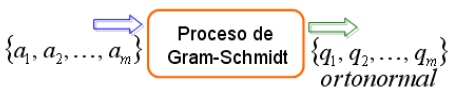
\includegraphics[scale=0.5]{gsproc.png}
 \end{center}}
 \end{frame}
 %%%%%
 \begin{frame}{Proceso de Gram-Schmidt}
  \begin{itemize}
   \item Paso 1: Tomando $\hat q_1= a_1$, se tiene que 
   \uncover<2->{$$
   q_1 = \frac{\hat q_1}{\|\hat q_1\|}
   $$
   \begin{center}
  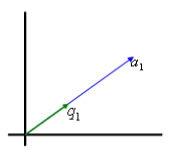
\includegraphics[scale=0.5]{gs_p1.png}
 \end{center}
 Se tiene as\'i que el conjunto $\{q_1\}$ es ortonormal.}
  \end{itemize}
 \end{frame}
 %%%%%%%
 \begin{frame}{Proceso de Gram-Schmidt}
 \begin{itemize}
  \item<1-> Paso 2: El objetivo es hallar $q_2$ tal que sea ortogonal a $q_1$, y adem\'as $q_2$ debe ser de tama\~no 1.  Es claro que el \'angulo entre $a_1$ y $a_2$ no necesariamente es de 90.
  \begin{center}
  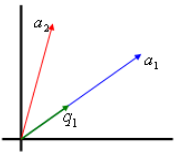
\includegraphics[scale=0.5]{gs_p2_a.png}
 \end{center}
 \item<2-> Considerando la proyecci\'on ortogonal de $a_2$ sobre $q_1$. Observese que el vector $\hat q_2=a_2-\alpha q_1$ es ortogonal a $q_1$
  \begin{center}
  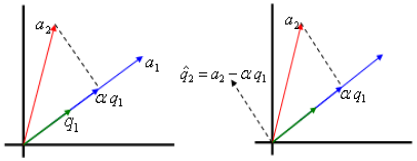
\includegraphics[scale=0.5]{gs_p2_b.png}
 \end{center}
 \end{itemize} 
 \end{frame}
 %%%%%%
 \begin{frame}{Proceso de Gram-Schmidt}
  \begin{itemize}
   \item Por lo tanto, $\alpha$ se debe elegir tal que $\hat q_2$ sea ortogonal a $q_1$, es 
 decir, debe ser tal que $\langle q_1,\hat q_2\rangle$ sea igual a cero:
   \begin{eqnarray}
    \nonumber 0 & = & \langle q_1,\hat q_2\rangle = \langle q_1,a_2-\alpha q_1\rangle \\
   \nonumber  & = & \langle q_1,a_2 \rangle - \langle q_1,\alpha q_1\rangle = \langle q_1,a_2 \rangle - \alpha \langle q_1,q_1\rangle\\
    \nonumber & = & \langle q_1,a_2 \rangle - \alpha 
   \end{eqnarray}
  \item<2-> De donde se obtiene que $\alpha=\langle q_1,a_2\rangle$.  As\'i que
  $$
  \hat q_2 = a_2 - \langle q_1,a_2\rangle q_1
  $$
  \item<3-> El vector $q_2$ ser\'a la normalizaci\'on de $\hat q_2$, es decir,
  $$
  q_2 = \frac{\hat q_2}{\|\hat q_2\|}
  $$
  \end{itemize}
 \end{frame}
 %%%%%%
 \begin{frame}{Proceso de Gram-Schmidt}
  \begin{itemize}
   \item Paso $j$: Tomando $a_j$ con $3\leq j \leq n$ del conjunto $\{a_1,a_2,\ldots,a_n\}$. El objetivo es hallar $q_j$ de tama\~no 1 tal que $\{q_1,q_2,\ldots,q_{j-1},q_j\}$ tambi\'en sea un conjunto ortonormal.  Del paso anterior se tiene construido al conjunto ortonormal $\{q_1,q_2,\ldots,q_{j-1}\}$
   \begin{eqnarray}
   \nonumber \hat q_j &=& a_j - \underbrace{\langle q_1,a_j\rangle}_{r_{1j}}q_1 - \underbrace{\langle q_2,a_j\rangle}_{r_{2j}}q_2 - \cdots - \underbrace{\langle q_{j-1},a_j\rangle}_{r_{j-1,j}}q_{j-1} \\
   \nonumber q_j &=& \frac{\hat q_j}{\|\hat q_j\|} = \frac{\hat q_j}{r_{jj}}
   \end{eqnarray}
  \end{itemize}
 \end{frame}
 %%%%%%
 \begin{frame}{Proceso de Gram-Schmidt}
  \begin{itemize}
   \item Se puede observar de las relaciones anteriores que
   $$
   \hat q_j = r_{jj}q_j
   $$
   \item<2-> Mientras que por otro lado
   $$
   a_j = \sum_{i=1}^{j-1}r_{ij}q_i + r_{jj}q_j = \sum_{i=1}^{j}r_{ij}q_i
   $$
  \end{itemize}
 \end{frame}
 %%%%%%
 \begin{frame}{Proceso de Gram-Schmidt}
 \begin{itemize}
  \item Si se consideran los vectores del conjunto $\{a_1,a_2,\ldots,a_n\}$ son las columnas de la matriz $A\in \mathbb{R}^{m\times n}$ y que adem\'as $\{q_1,q_2,\ldots,q_n\}$ son las columnas de la matriz $Q\in \mathbb{R}^{m \times n}$ entonces esta \'ultima expresi\'on es de mucha utilidad para obtener la factorizaci\'on $QR$ de $A$. Para identificar la matriz triangular $R$ bastan unas pocas observaciones.
  \item<2-> Para $j=1$
  $$
  a_1 = r_{11}q_1 = r_{11}q_1 + 0q_2 + \cdots + 0q_n = Q\left[\begin{array}{c}
                                                               r_{11}\\
                                                               0\\
                                                               \vdots\\
                                                               0
                                                              \end{array}\right] = Qr_1
  $$
 \end{itemize}
 \end{frame}
 %%%%%
 \begin{frame}{Proceso de Gram-Schmidt}
 \begin{itemize}
 \item Para $j=2$
 \footnotesize
  $$
  a_2 = r_{12}q_1 + r_{22}q_2 = r_{12}q_1+ r_{22}q_2 + 0q_3 + \cdots + 0q_n = Q\left[\begin{array}{c}
                                                               r_{12}\\
                                                               r_{22}\\
                                                               0\\
                                                               \vdots\\
                                                               0
                                                              \end{array}\right] = Qr_2
  $$
  \normalsize
  \item Para $j=k$
  \scriptsize
  $$
  a_k = r_{1k}q_1 + \cdots + r_{kk}q_k = r_{1k}q_1+ \cdots + r_{kk}q_k + 0q_{k+1} + \cdots + 0q_n = Q\left[\begin{array}{c}
                                                               r_{1k}\\
                                                               \vdots\\
                                                               r_{kk}\\
                                                               0\\
                                                               \vdots\\
                                                               0
                                                              \end{array}\right] = Qr_k
  $$
  \normalsize
 \end{itemize}
 \end{frame}
 %%%%%
 \begin{frame}{Proceso de Gram-Schmidt}
  \begin{itemize}
   \item Para $j=n$
   $$
  a_n = r_{1n}q_1 + \cdots + r_{nn}q_n  = Q\left[\begin{array}{c}
                                                               r_{1n}\\
                                                               \vdots\\
                                                               r_{nn}\\                                                              
                                                              \end{array}\right] = Qr_n
  $$
  \item<2-> Finalmente, si se escriben todas estas expresiones de forma matricial se obtiene que
  $$
  A = [a_1 a_2 \cdots a_n] = [Qr_1 Qr_2 \cdots Qr_n] = Q[r_1 r_2 \cdots r_n] = QR
  $$
  \end{itemize}
 \end{frame}
 %%%%%%
 \begin{frame}{Algoritmo}
 \begin{block}{C\'odigo 1}
 %\scriptsize
 \texttt{
 \hspace{-0.25cm}\textcolor{blue}{function} [Q,R]=my\_gram\_schmidt(A)\\
 m=size(A,1); n=size(A,2); Q=zeros(m,n); R=zeros(n);\\
 \textcolor{blue}{for} j=1:n\\
 \hspace{0.25cm} v=A(:,j);\\
 \hspace{0.25cm} \textcolor{blue}{for} i=1:j-1\\
 \hspace{0.5cm} R(i,j) = Q(:,i)'*A(:,j);\\
 \hspace{0.5cm} v = v - R(i,j)*Q(:,i);\\
 \hspace{0.25cm} \textcolor{blue}{end}\\
 \hspace{0.25cm} R(j,j) = norm(v);\\
 \hspace{0.25cm} Q(:,j) = v/R(j,j);\\
 \textcolor{blue}{end}
 }
 \end{block}
 \end{frame}
 %%%%%
\begin{frame}{Gram Schmidt Modificado}
  \begin{itemize}
   \item En la pr\'actica, la p\'erdida de ortogonalidad de los vectores $q_i$ que se van calculando en el proceso de Gram Schmidt es m\'as que evidente, debido a errores de redondeo y de cancelaci\'on si, por ejemplo, alguno de los vectores columna $a_j$ est\'a pr\'oximo al subespacio generado por los vectores anteriores $q_1, \ldots q_{j-1}$.
   \item<2-> En ese caso, los sumandos de la expresi\'on $a_j - \sum_{i=1}^{j-1}\langle q_i,a_j\rangle q_i$ pueden llegar a ser muy peque\~nos o muy distantes unos de otros, si bien el resultado final puede ser muy peque\~no, por lo que el error num\'erico que se va produciendo es relativamente grande. Al dividir el resultado por su norma (tambi\'en muy peque\~na) los errores se amplificar\'an a\'un m\'as.
  \end{itemize}
  \end{frame}
  %%%%%%
  \begin{frame}{Gram Schmidt Modificado}
   \begin{itemize}
    \item En 1966 Rice modific\'o el m\'etodo haciendo que en una etapa $k$, en vez de sustraer del vector $a_k$ sus coeficientes sobre todos los $k-1$ vectores $q_i$ ya calculados, $q_k$ se hace igual a $a_k$ al principio y luego se le van sustrayendo su proyecci\'on en $q_1$, pasando a ser el nuevo $q_k$ el resultado, el cual se proyecta luego en $q_2$, y as\'i sucesivamente en cada uno de los $k-1$ $q_i$ anteriores. 
    \item<2-> El resultado con esta simple nueva disposici\'on de los c\'alculos es indiscutiblemente mejor num\'ericamente.
   \end{itemize}
  \end{frame}
  %%%%%%%
  \begin{frame}{Algoritmo}
  \begin{block}{C\'odigo 2}
  %\scriptsize
  \texttt{
  \hspace{-0.25cm}\textcolor{blue}{function} [Q,R]=my\_gram\_schmidt\_mod(A)\\
  m=size(A,1); n=size(A,2); Q=zeros(m,n); R=zeros(n);\\
  \textcolor{blue}{for} j=1:n\\
  \hspace{0.25cm} v=A(:,j);\\
  \hspace{0.25cm} \textcolor{blue}{for} i=1:j-1\\
  \hspace{0.5cm} R(i,j) = Q(:,i)'*v;\\
  \hspace{0.5cm} v = v - R(i,j)*Q(:,i);\\
  \hspace{0.25cm} \textcolor{blue}{end}\\
  \hspace{0.25cm} R(j,j) = norm(v);\\
  \hspace{0.25cm} Q(:,j) = v/R(j,j);\\
  \textcolor{blue}{end}
  }
  \end{block}
  \end{frame}
  %%%%%%%
  \begin{frame}
    \frametitle{Ejemplo}
    Considere la matriz
    $$
    A = \left(\begin{array}{ccc}
      1 & 1 & 0\\
      1 & 0 & 1\\
      0 & 1 & 1
    \end{array}\right)
    $$
    con vectores $a_1 =(1, 1, 0)^T$, $a_2 =(1, 0, 1)^T$ y $a_3 =(0, 1, 1)^T$
    \vspace{1cm}

    Aplicando el procedimiento de Gram-Schmidt se obtienen los siguientes resultados:
  \end{frame}
  %%%%
  \begin{frame}
    \frametitle{Ejemplo}
    \begin{eqnarray}
      \nonumber \hat{q}_1 &=& a_1 =(1, 1, 0)^T\\
      \uncover<2->{\nonumber q_1 &=& \frac{\hat{q}_1}{\|\hat{q}_1\|} = \frac{1}{\sqrt{2}}(1, 1, 0)^T = \left(\frac{1}{\sqrt{2}}, \frac{1}{\sqrt{2}}, 0\right)^T}\\
      \uncover<3->{\nonumber \hat{q}_2 &=& a_2-\langle a_2,q_1\rangle q_1 =(1,0, 1)^T-\frac{1}{\sqrt{2}}\left(\frac{1}{\sqrt{2}}, \frac{1}{\sqrt{2}}, 0\right)^T\\
      \nonumber &=& \left(\frac{1}{2}, -\frac{1}{2}, 1\right)^T}\\
      \uncover<4->{\nonumber q_2 &=& \frac{\hat{q}_2}{\|\hat{q}_2\|} = \frac{1}{\sqrt{3/2}}\left(\frac{1}{2}, -\frac{1}{2}, 1\right)^T = \left(\frac{1}{\sqrt{6}}, -\frac{1}{\sqrt{6}}, \frac{2}{\sqrt{6}}\right)^T}
    \end{eqnarray}
  \end{frame}
  %%%%
  \begin{frame}
    \frametitle{Ejemplo}
    \begin{eqnarray}
      \nonumber \hat{q}_3 &=& a_3-\langle a_3,q_1\rangle q_1 - \langle a_3,q_2\rangle q_2 = (0, 1, 1)^T-\frac{1}{\sqrt{2}}\left(\frac{1}{\sqrt{2}}, \frac{1}{\sqrt{2}}, 0\right)^T\\
      \nonumber & &-\frac{1}{\sqrt{6}}\left(\frac{1}{\sqrt{6}}, -\frac{1}{\sqrt{6}}, \frac{2}{\sqrt{6}}\right)^T = \left(-\frac{1}{\sqrt{3}}, \frac{1}{\sqrt{3}}, \frac{1}{\sqrt{3}}\right)^T\\
      \uncover<2->{\nonumber q_3 &=& \frac{\hat{q}_3}{\|\hat{q}_3\|} = \left(-\frac{1}{\sqrt{3}}, \frac{1}{\sqrt{3}}, \frac{1}{\sqrt{3}}\right)^T}
    \end{eqnarray}
  \end{frame}
  %%%%
  \begin{frame}
    \frametitle{Ejemplo}
    Entonces la matriz $Q$ obtenida es
    $$
    Q = \left(q_1, q_2, \cdots, q_n\right) = \left(\begin{array}{ccc}
      \dfrac{1}{\sqrt{2}} & \dfrac{1}{\sqrt{6}} & -\dfrac{1}{\sqrt{3}}\\
      \dfrac{1}{\sqrt{2}} & -\dfrac{1}{\sqrt{6}} & \dfrac{1}{\sqrt{3}}\\
       0 & \dfrac{2}{\sqrt{6}} & \dfrac{1}{\sqrt{3}}
    \end{array}\right)
    $$
    Mientras que la matriz $R$ obtenida es
    $$
    R = \left(\begin{array}{ccc}
      \langle a_1,q_1\rangle & \langle a_2,q_1\rangle & \langle a_3,q_1\rangle\\
      0 & \langle a_2,q_2\rangle & \langle a_3,q_2\rangle \\
      0 & 0 & \langle a_3,q_3\rangle
    \end{array}\right) = \left(\begin{array}{ccc}
      \dfrac{2}{\sqrt{2}} & \dfrac{1}{\sqrt{2}} & \dfrac{1}{\sqrt{2}}\\
       0 & \dfrac{3}{\sqrt{6}} & \dfrac{1}{\sqrt{6}}\\
       0 & 0 & \dfrac{2}{\sqrt{3}}
    \end{array}\right)
    $$
  \end{frame}      
%%%%%%%
\begin{frame}{Ejercicio}
  \begin{enumerate}
   \item Implemente la factorizaci\'on $QR$ via Gram Schmidt.
   \item Ejecute ambos c\'odigos con la matriz
   $$
   A = \left[\begin{array}{ccc}
              -2 & 3 & 1\\
              1 & -1 & 1\\
              2 & -1 & 4\\
              -2 & 2 & 1
             \end{array}\right]
   $$
   \item Escriba en la ventana de comandos
  \begin{center}
  \texttt{
    \begin{tabular}{l}
     >> Q*R\\
     >> Q'*Q - eye(3)
    \end{tabular}}
   \end{center}
   \item Realice las mismas comprobaciones para la siquiente matriz
   $$
   A = \left[\begin{array}{ccc}
              1 & 1 & 1\\
              \epsilon & 0 & 0\\
              0 & \epsilon & 0\\
              0 & 0 & \epsilon
             \end{array}\right], \qquad \epsilon = 10^{-9}
   $$
  \end{enumerate}
 \end{frame}
 %%%%%
\begin{frame}{Reflexi\'on de Householder}
  \begin{itemize}
    \item Considerese un espacio vectorial de dimensiones $n$ definido sobre un cuerpo $\mathbb{K}$, y se denotar\'a por $\mathbb{K}^n$ (En general $\mathbb{R}^n$ o $\mathbb{C}^n$).
    \item<2-> Dado un vector $u \in \mathbb{K}^n$, se define la transformaci\'on $H$ de Householder asociada al vector $u$ a la que viene definida por la matriz:
  $$
  H = \begin{cases}
    I - 2\dfrac{uu^*}{u^*u} & \mbox{ si } u \neq 0\\
    I \in \mathbb{K}^{n\times n} & \mbox{ si } u = 0
  \end{cases}
  $$
\end{itemize}
\end{frame}
%%%%%
\begin{frame}{Reflexi\'on de Householder}
  \begin{block}{Proposici\'on}
    La transformaci\'on de Householder $H$ asociada al vector $u \in \mathbb{K}^n$ posee las siguientes propiedades:
    \begin{enumerate}
      \item<2-> $H$ es herm\'itica ($H^*=H$).
      \item<3-> $H$ es unitaria ($H^*H = HH^* = I$).
      \item<4-> $H^2 = I$ o lo que es igual, $H^{-1}=H$.
    \end{enumerate}
  \end{block}
\end{frame}
%%%%% 
\begin{frame}{Reflexi\'on de Householder}
  Demostraci\'on:
  \begin{enumerate}
    \item<2-> $H^* = \left(I-2\dfrac{uu^*}{u^*u}\right)^* = \left(I-2\dfrac{u^*u}{u^*u}\right) = I-2\dfrac{uu^*}{u^*u} = I-2\dfrac{(uu^*)^*}{u^*u} = I-2\dfrac{uu^*}{u^*u} = H$.
    \item<3-> $HH^* = HH = \left(I-2\dfrac{uu^*}{u^*u}\right)\left(I-2\dfrac{uu^*}{u^*u}\right) = I-4\dfrac{uu^*}{u^*u} + 4\dfrac{uu^*uu^*}{(u^*u)^2} = I-4\dfrac{uu^*}{u^*u} + 4\dfrac{u(u^*u)u^*}{(u^*u)^2} = I-4\dfrac{uu^*}{u^*u} + 4\dfrac{uu^*}{u^*u} = I$
    \item<4-> De los dos puntos anteriores se deduce que $ H^2= HH = HH^* = I$.
  \end{enumerate}
\end{frame}
%%%%%
\begin{frame}{Reflexi\'on de Householder}
  \textbf{Interpretaci\'on Geom\'etrica en $\mathbb{R}^n$}
  \begin{itemize}
   \item Sean $u \in \mathbb{R}^n$ un vector tal que $\|u\|_2=1$ y $H$ la transformaci\'on de Householder asociado a \'el:
   $$
   H = I - 2uu^t
   $$
   \item<2-> Si $x \in \mathbb{R}^n$ entonces
   \begin{eqnarray}
    \nonumber Hx & = & (I - 2uu^t)x = x - 2uu^tx = x-2u\langle x,u\rangle=\\
      \nonumber & = & x-2u(\|x\|\|u\|\cos(\alpha)) = x-2u(\|x\|\cos(\alpha))=\\
    \nonumber & = & x-2\lambda u \qquad \mbox{  con  }\qquad \lambda=\|x\|\cos(\alpha)
    \end{eqnarray}
    donde $\alpha$ representa el \'angulo que forman los vectores $x$ y $u$.
  \end{itemize}
\end{frame}   
%%%%
\begin{frame}{Reflexi\'on de Householder}
  \begin{itemize}
   \item<1-> Sea $y$ el vector sim\'etrico de $x$ respecto del hiperplano perpendicular a $u$.
   \begin{center}
     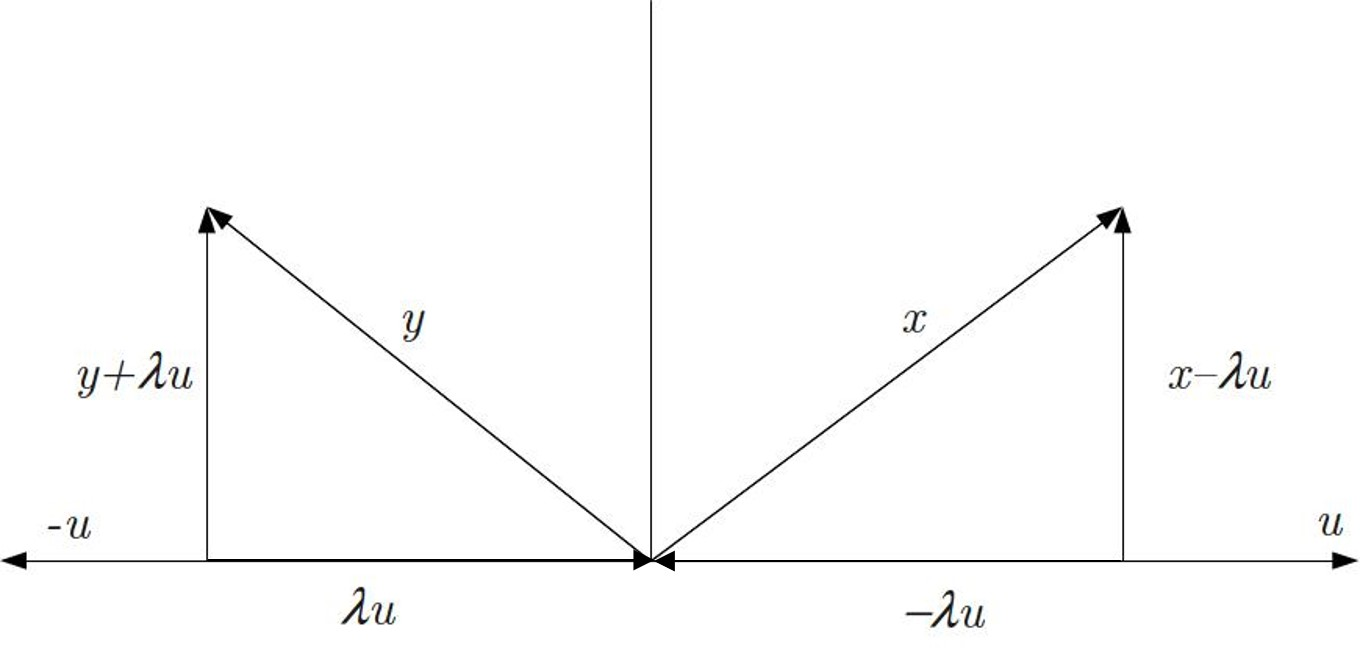
\includegraphics[scale=0.3]{./reflex.jpg}\\
     Un vector $x$ y su transformado $y=Hx$.
   \end{center}   
   \item<2-> Se puede observar que 
   $$
   y + \lambda u = x - \lambda u \Longleftrightarrow y = x-2\lambda u = Hx
   $$
  \end{itemize}
\end{frame}
%%%%
\begin{frame}{Reflexi\'on de Householder}
  \begin{itemize}
   \item<1-> Dado un vector $x\neq 0$, es sencillo hallar la reflexi\'on de Householder $H=I-2uu^t$ que anula las entradas de $x$ con excepci\'on de la primera entrada, es decir:  
$$
Hx = x - 2(u^tx)u = \left(\begin{array}{cccc}
                           c & 0 & 0 & \cdots                           
                          \end{array}\right)^t=ce_1
$$

\item<2-> Dado que $H$ es ortogonal, $|c|=\|Hx\|=\|x\|$, se puede escribir:
$$
u = \frac{1}{2u^tx}(x-ce_1)
$$

es decir, $u$ debe ser paralelo al vector $\tilde u=x\pm\|x\|e_1$, por lo tanto
$$
\displaystyle u = \frac{x \pm \|x\|e_1}{\|x \pm \|x\|e_1\|}
$$
\end{itemize}
\end{frame}
%%%%
\begin{frame}{Reflexi\'on de Householder}
  \begin{itemize}
    \item Independientemente de la elecci\'on del signo se mantiene que $u$ satisface $Hx=ce_1$ siempre que $\tilde u \neq 0$.
    \item<2-> empleando la siguiente expresi\'on $\tilde u = x + sign(x_1)\|x\|e_1$ para evitar la cancelaci\'on en la primera componente de $\tilde u$, se obtiene el siguiente resultado:
    $$
    \tilde u =\left(\begin{array}{c}
                     x_1 + sign(x_1)\|x\|\\
                     x_2\\
                     \vdots\\
                     x_n
                    \end{array}
    \right) \mbox{ con } u=\frac{\tilde u}{\|\tilde u\|}
    $$
    \item<3->El correspondiente vector de Householder es
$$
H(x) = I-2uu^t = I - \frac{2\tilde u\tilde u^t}{\|\tilde u\|^2}
$$    
  \end{itemize}
\end{frame}
%%%%
\begin{frame}{Reflexi\'on de Householder}
  \begin{itemize}
    \item<1-> Dada una matriz $A_{m\times n}$, se puede obtener una matriz triangular superior multiplicando por la izquierda de manera apropiada por
    matrices de Householder. Asumiendo que ninguna de las columnas de $A$ es completamente cero.
    \item<2-> Esto puede llevarse a cabo con una matriz de Householder, la cual denotamos por $H(a_1)$. De esta manera:
    $$
    A_1 = H(a_1)A = \left(\begin{array}{ccccc}
                           *&*&*&\cdots&*\\
                           0&\underline{*}&*&\cdots&*\\                           
                           \vdots&\vdots&\vdots&& \vdots\\
                           0&\underline{*}&*&\cdots&*\\    
                          \end{array}
    \right)
    $$    
    Denotemos $H_1=H(a_1)$ por simplicidad.  
  \end{itemize}
\end{frame}
%%%%
\begin{frame}{Reflexi\'on de Householder}
  \begin{itemize}
    \item<1-> Tomando la segunda columna de $A_1=H(a_1)A$ y obviando la primera primera entrada, para ello consideraremos el vector
    $\tilde a_2$ de tama\~no $n-1$.    
    \item<2-> Si $\tilde a_2$ posee elementos no nulos por debajo de la entrada superior, entonces la reflexi\'on  de Householder
    $H_2=H(\tilde a_2)$ viene dada por la siguiente matriz.    
    $$
    H_2 = \left(\begin{array}{c|cccc}
                 1      & 0 & 0               & \cdots & 0 \\\hline
                 0      &   &                 &        &\\
                 \vdots &   & H(\tilde {a_2}) &        &\\
                 0      &   &                 &        &
                \end{array}
     \right)
    $$
    \end{itemize}
\end{frame}
%%%%
\begin{frame}{Reflexi\'on de Householder}
    Y al realizar el producto se obtiene el siguiente resultado    
    $$
    A_2 = H_2A_1 = \left(\begin{array}{cccccc}
                           *&*&*&*&\cdots&*\\
                           0&*&*&*&\cdots&*\\
                           0&0&\underline{*}&*&\cdots&*\\
                           0&0&\underline{*}&*&\cdots&*\\
                           \vdots&\vdots&\vdots&\vdots&& \vdots\\
                           0&0&\underline{*}&*&\cdots&*\\
                          \end{array}
    \right)
    $$
\end{frame}
%%%%%
%%%%%
\begin{frame}{Reflexi\'on de Householder}
  \begin{itemize}
    \item<1-> Considerando la siguiente columna de $A_2$ la cual contiene elementos no nulos debajo de la tercera
    fila. Obviando las dos entradas superiores y considerando al vector $\tilde a_3$ de
    tama\~no $n-2$ 
    \item<2-> Se puede obtener el reflector de Householder $H(\tilde a_3)\in
    \mathbb{R}^{n-2}$, y multiplicando a $A_2$ por la izquierda con
    $$
    H_3 = \left(\begin{array}{cc|ccc}
      1      & 0      & 0 & \cdots           & 0 \\
      0      & 1      & 0 & \cdots           & 0 \\\hline
      0      & 0      &   &                  & \\
      \vdots & \vdots &   &  H(\tilde {a_3}) &\\
      0      & 0      &   &                  &
     \end{array}
\right)
    $$
    obteniendo como resultado la mattriz $A_3 = H_3A_2$ triangular superior en sus primeras tres columnas.
  \end{itemize}
\end{frame}
%%%%
\begin{frame}{Reflexi\'on de Householder}
  \begin{itemize}
    \item<1-> A lo sumo en $(n-1)$ pasos se obtiene una matriz triangular superior $R$, producto de la aplicaci\'on de
    matrices de reflexi\'on de Householder, se tiene entonces que:
    $$
    H_{n-1}H_{n-2}\cdots H_2H_1A=R
    $$
    \item<2-> Las matrices $H_i$ son matrices ortogonales, por lo tanto:    
    $$
    A=QR
    $$    
    con    
    $$
    Q=H_1H_2\cdots H_{n-2}H_{n-1}
    $$
    \end{itemize}
\end{frame}
%%%%
\begin{frame}{Ejemplo:}
  Hallar la factorizaci\'on $QR$ de $A=\left(\begin{array}{ccc}
    1 & 2 & 3\\
    0 & 3 & 2\\
    2 & 0 & 1
   \end{array}\right)$ mediante reflexiones de Householder.

   \uncover<2->{
    La primera columna de $A$ es $a_1=\left(\begin{array}{c}
    1\\
    0\\
    2
   \end{array}
\right)$.}

\uncover<3->{Por lo que el correspondiente vector de Householder es   
$$
\tilde u = \left(\begin{array}{c}
1+\sqrt{5}\\
0\\
2
\end{array}\right)
$$

con norma cuadrada $\|\tilde u\|^2= 10+2\sqrt{5}$}
\end{frame}
%%%%%
%%%%
\begin{frame}{Ejemplo:}
  Por lo tanto:
  $$
  H_1=H(a_1) = I - \frac{2\tilde u \tilde u^t}{10+2\sqrt{5}} = \left(\begin{array}{ccc}
                                                                    -\dfrac{1}{\sqrt{5}} & 0 & -\dfrac{2}{\sqrt{5}}\\
                                                                    0 & 1 & 0\\
                                                                    -\dfrac{2}{\sqrt{5}} & 0 & \dfrac{1}{\sqrt{5}}
                                                                   \end{array}\right)
$$

\uncover<2->{
por lo que
$$
A_1 =H_1A = \displaystyle\left(\begin{array}{ccc}
                               -\sqrt{5} & -\dfrac{2}{\sqrt{5}} & \sqrt{5}\\
                               0 & 3 & 2\\
                               0 & -\dfrac{4}{\sqrt{5}} & \sqrt{5}
                               \end{array}\right)
$$}
\end{frame}
%%%%%
\begin{frame}{Ejemplo:}
El pr\'oximo vector columna es
$$
\tilde a_2 = \left(\begin{array}{c}
                    3\\
                    -\dfrac{4}{\sqrt{5}}
                   \end{array}\right)
$$

cuya norma es $\|\tilde a_2\|= \sqrt{\dfrac{61}{5}}$ \uncover<2->{y el correspondiente vector de Householder es
$$
\tilde u = \left(\begin{array}{c}
                    3+\sqrt{\dfrac{61}{5}}\\
                    -\dfrac{4}{\sqrt{5}}
                   \end{array}\right)=\left(\begin{array}{c}
                   6.492\\
                   -1.788
                   \end{array}\right)
$$

cuya norma cuadrada es $\|\tilde u\|^2= 45.346$.}
\end{frame}
%%%%%%
\begin{frame}{Ejemplo:}
Por lo tanto:
$$  
H_2=H(\tilde a_2) = I - \frac{2\tilde u \tilde u^t}{45.346} = 
\left(\begin{array}{cc}
  -0.8589 &  0.5121\\
  0.5121 &  0.8589 \\
  \end{array}\right)
$$
Por lo que la matriz de Householder $3 \times 3$ es
$$
H_2 = \left(\begin{array}{ccc}
      1 & 0 & 0\\
      0 & -0.8589 & 0.5122\\
      0 & 0.5122 & 0.8589
      \end{array}\right)
$$
cuya aplicaci\'on a $A_1$ es
$$
A_2 = H_2A_1 = \left(\begin{array}{ccc}
      -2.2361 & -0.8944 & -2.2361\\
      0 & -3.4928 & -2.8630\\
      0 & 0 & -0.8962
      \end{array}\right)
$$
\end{frame}
%%%%%%
\begin{frame}{Ejemplo:}
  Esta es la matriz $R$ de la factorizaci\'on $QR$. Para obtener $Q$ se computa
  $$
  Q=H_1H_2 = \left(\begin{array}{ccc}
    -0.4472 &  -0.4581 & -0.7682\\
        0 & -0.8589 & 0.5122\\
  -0.8944 &  0.2290 & 0.3841
        \end{array}\right)
  $$

  Por lo tanto la factorizaci\'on $QR$ de $A$ es
  \scriptsize{
  $$
  A = QR = \left(\begin{array}{ccc}
    -0.4472 &  -0.4581 & -0.7682\\
        0 & -0.8589 & 0.5122\\
  -0.8944 &  0.2290 & 0.3841
        \end{array}\right) \left(\begin{array}{ccc}
    -2.2361 & -0.8944 & -2.2361\\
    0 & -3.4928 & -2.8630\\
    0 & 0 & -0.8962
        \end{array}\right)
  $$}
  \normalsize
  $$
  = \left(\begin{array}{ccc}
    1 &  2 & 3\\
        0 & 3 & 2\\
  2 &  0 & 1
        \end{array}\right)
  $$
\end{frame}
%%%%%
\begin{frame}{Algoritmo}
  \begin{block}{C\'odigo}
%\scriptsize
\texttt{
\hspace{-0.25cm}\textcolor{blue}{function} [Q,R]=my\_householder\_QR(A)\\
m=size(A,1); n=size(A,2); Q=eye(m); R=A; I=eye(m);\\
\textcolor{blue}{for} j=1:n\\
\hspace{0.25cm} x = R(j:m,j);\\
\hspace{0.25cm} v = -sign(x(1))*norm(x)*eye(m-j+1,1)-x;\\
\hspace{0.25cm} \textcolor{blue}{if} norm(v)>0\\
\hspace{0.5cm} v = v/norm(v);\\
\hspace{0.5cm} P = I;\\
\hspace{0.5cm} P(j:m,j:m) = P(j:m,j:m)-2*v*v';\\
\hspace{0.5cm} R = P*R;\\
\hspace{0.5cm} Q = Q*P;\\
\hspace{0.25cm} \textcolor{blue}{end}\\
\textcolor{blue}{end}
}
\end{block}
\end{frame}
%%%%%
\begin{frame}
  \frametitle{Rotaciones de Givens}
  \begin{itemize}
    \item La descomposici\'on $QR$ tambi\'en puede ser calculada mediante una serie de rotaciones de Givens.
    \item<2-> Cada rotaci\'on anula un elemento por debajo de la diagonal de la matriz, para formar la matriz $R$.
    \item<3-> La concatenaci\'on de todas las matrices de rotaci\'on de Givens conforman la matriz ortogonal $Q$.
    \item<4-> Al igual que en Householder, la idea es calcular matrices ortogonales $Q_1,Q_2,\ldots,Q_k$ usando rotaciones de Givens tales que: $A^{(1)}=Q_1A$ tiene ceros debajo de la entrada $(1,1)$ en la primera columna.
    \item<5-> Luego construir $Q_2$ tal que $A^{(2)}=Q_2A^{(1)}$ tenga ceros debajo de la posici\'on $(2,2)$ en la segunda columna y as\'i sucesivamente hasta $A^{(s)}=Q_sA^{(s-1)}$.
  \end{itemize}
\end{frame}
%%%%%
\begin{frame}
  \frametitle{Descomposici\'on $QR$}
  Una matriz de la forma

  \begin{eqnarray}
  \nonumber\begin{array}{cccccccc}
    i &  &  j &         &        &        &       & \mbox{columnas}\\
   \downarrow&   &  \downarrow &         &       &        &       &
  \end{array}\\
  \nonumber J(i,j,\theta) =\left(\begin{array}{cccccccc}
  1 & 0 & 0 & \cdots & \cdots & \cdots & \cdots & 0\\
  0 & 1 & 0 & \cdots & \cdots & \cdots & \cdots & 0\\
  \vdots & \vdots & \vdots &  &  &  & \cdots & \vdots\\
  0 & 0 & 0 & \cdots & c & s & \cdots & 0\\
  \vdots & \vdots & \vdots &  &  &  & \cdots & \vdots\\
  0 & 0 & 0 & \cdots & -s & c & \cdots & 0\\
  \vdots & \vdots & \vdots &  &  &  & \cdots & \vdots\\
  0 & 0 & 0 & \cdots & \cdots & 0 & \cdots & 1\\
  \end{array}\right)\begin{array}{c}
  \\
  \\
  \\
  \leftarrow i\\
  filas \\ 
  \leftarrow j\\
  \\
  \\
  \end{array}
  \end{eqnarray}
  
  donde $c^2+s^2=1$ es denominada matriz de Givens, para un cierto $\theta$.
\end{frame} 
%%%%%%
\begin{frame}
  \frametitle{Rotaciones de Givens}
  \textbf{Interpretaci\'on Geom\'etrica.}
  \begin{itemize}
    \item<2-> La matriz $J(i,j,\theta)$ rota un par de ejes coordenados en \'angulo $\theta$ en el plano $(i,j)$. 
    \item<3-> La matriz $J(i,j,\theta)$ es comunmente conocida como una rotaci\'on de Givens o rotaci\'on en el plano $(i,j)$.
     \begin{figure}[h]
      \begin{center}
        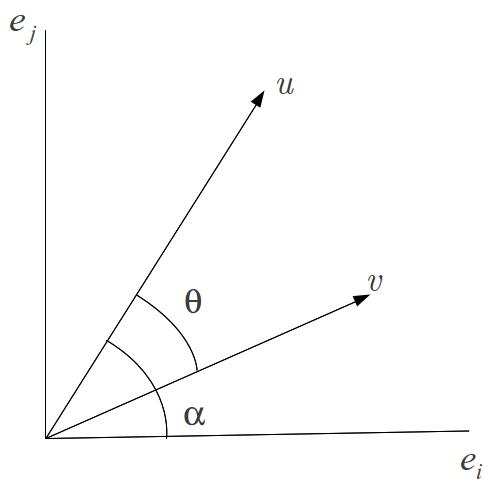
\includegraphics[scale=0.2]{./rotacion.jpg}
      \end{center}
      \caption{Un vector $u$ y su transformado $v$ por rotaci\'on.}
      \label{rotacion}
      \end{figure}
  \end{itemize}
\end{frame}
%%%%
\begin{frame}
  \frametitle{Rotaciones de Givens}
  \begin{itemize}
    \item<1-> De la gr\'afica se puede observar que $u=(\cos(\alpha),\sin(\alpha))$ y $v=(\cos(\alpha - \theta),\sin(\alpha-\theta))$.
    \uncover<2->{    
    \begin{eqnarray}
    \nonumber \cos(\alpha - \theta) & = & \cos(\alpha)\cos(-\theta) - \sin(\alpha)\sin(-\theta)\\
    \nonumber & = & \cos(\alpha)\cos(\theta) -\sin(\alpha)(-\sin(\theta))\\
    \nonumber & = & \cos(\alpha)\cos(\theta) +\sin(\alpha)\sin(\theta)
    \end{eqnarray}}
    \uncover<3->{
    \begin{eqnarray}
    \nonumber \sin(\alpha - \theta) & = & \sin(\alpha)\cos(-\theta) + \cos(\alpha)\sin(-\theta)\\
    \nonumber & = & \sin(\alpha)\cos(\theta) +\cos(\alpha)(-\sin(\theta))\\
    \nonumber & = & \sin(\alpha)\cos(\theta) -\cos(\alpha)\sin(\theta)
    \end{eqnarray}}
  \end{itemize}    
\end{frame}
%%%%%
\begin{frame}
  \frametitle{Rotaciones de Givens}
  \begin{itemize}
    \item<1-> Por lo tanto 

    \begin{eqnarray}
     \nonumber v & = & \left(\begin{array}{c}
                        \cos(\alpha - \theta)\\
                        \sin(\alpha - \theta)
                        \end{array}\right) = 
                        \left(\begin{array}{c}
                        \cos(\alpha)\cos(\theta) +\sin(\alpha)\sin(\theta)\\
                        \sin(\alpha)\cos(\theta) -\cos(\alpha)\sin(\theta)
                        \end{array}\right)\\
    \uncover<2->{\nonumber & = & \left(\begin{array}{cc}
                           \cos(\theta) & \sin(\theta)\\
                          -\sin(\theta) & \cos(\theta)
                          \end{array}\right)\left(\begin{array}{c}
                        \cos(\alpha)\\
                        \sin(\alpha)
                       \end{array}\right) }\\
    \uncover<3->{\nonumber\Rightarrow v & = &  \left(\begin{array}{cc}
                           \cos(\theta) & \sin(\theta)\\
                          -\sin(\theta) & \cos(\theta)
                          \end{array}\right)u}
    \end{eqnarray}
  \end{itemize}
\end{frame}  
%%%%
\begin{frame}
  \frametitle{Rotaciones de Givens}
  \begin{itemize}
    \item<1-> Para la construcci\'on de la matriz $J(i,j,\theta)$, sea 
    $x=\left(\begin{array}{c}
      x_1\\
      x_2
     \end{array}\right) \in \mathbb{R}^2$

\begin{center}
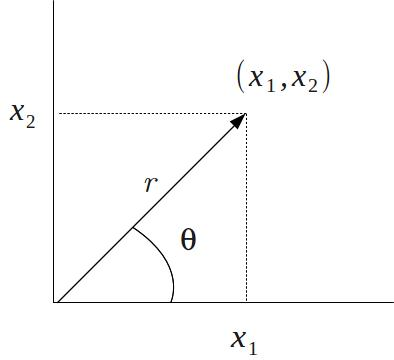
\includegraphics[scale=0.35]{./rota2.jpg}\\
Construcci\'on de la Matriz $J(i,j,\theta)$.
\end{center}
  \end{itemize}
\end{frame}
%%%%%
\begin{frame}
  \frametitle{Rotaciones de Givens}
  De la figura se pude observar que:
\begin{eqnarray}
\nonumber & \cos(\theta) = \dfrac{x_1}{r} \quad\quad \sin(\theta) = \dfrac{x_2}{r}\\
\nonumber & \cos^2(\theta) + \sin^2(\theta) = 1 \Rightarrow \left(\dfrac{x_1}{r}\right)^2 + \left(\dfrac{x_2}{r}\right)^2 = 1\\
\nonumber & c = \dfrac{x_1}{\sqrt{x_1^2+x_2^2}}, \quad\quad s=\dfrac{x_2}{\sqrt{x_1^2+x_2^2}} 
\end{eqnarray}
\end{frame} 
%%%%%
\begin{frame}
\frametitle{Rotaciones de Givens} 
\begin{itemize}
\item<1-> Por lo tanto:
$$
J(1,2,\theta) = \left(\begin{array}{cc}
                       c & s\\
		                  -s & c
                      \end{array}\right)
$$

\item<2->La matriz $J(1,2,\theta)$ es tal que:
$$
J(1,2,\theta)x = \left(\begin{array}{c}
                      *\\
		                  0
                      \end{array}\right) \mbox{ es m\'ultiplo de $e_1$ en $\mathbb{R}^2$}
$$
\end{itemize}  
\end{frame} 
%%%%%%
\begin{frame}{Rotaciones de Givens}
  \begin{itemize}
   \item Rotaciones de Givens pueden ser aplicadas de manera sistem\'atica a un par de filas de la matriz $A$ y as\'i 
 anular elementos hasta obtener una matriz triangular superior $R$.
 \item<2-> Elementos por debajo de la subdiagonal pueden ser anulados bajo distinto orden, pero se 
 deben preservar los 
 ceros realizados.
 \item<3-> Cada rotaci\'on debe ser aplicada a todos los elementos de las filas seleccionadas, no solo a las entradas que
 determinan $c$ y $s$
 \item<4-> Una vez obtenida la triangular superior, el producto de las matrices de rotaci\'on determina la matriz 
 ortogonal $Q$ de modo que $QR=A$
  \end{itemize}
 \end{frame}
 %%%%%%%
 \begin{frame}{Rotaciones de Givens}
  El c\'alculo de los valores de $c$ y $s$ puede causar overflow o underflow, y para su c\'alculo se comparan los 
 valores $x_1$ y $x_2$ seleccionados de la siguiente manera
 \begin{enumerate}
  \item<2-> Si $|x_2|\geq|x_1|$, entonces
  $$
  t = \dfrac{x_1}{x_2}, \qquad s=\dfrac{1}{\sqrt{1+t^2}}, \qquad c=st
  $$
  \item<3-> Si $|x_2|<|x_1|$, entonces
  $$
  t = \dfrac{x_2}{x_1}, \qquad c=\dfrac{1}{\sqrt{1+t^2}}, \qquad s=ct
  $$
 \end{enumerate}
 \end{frame}
%%%%%
\begin{frame}{Rotaciones de Givens} 
  \begin{itemize}
   \item<1->Ejemplo: Sea $x=\left(\begin{array}{c}
    1\\
    1/2
   \end{array}\right)$
   \item<2->En este caso $|x_1|=1 > |x_2|=1/2$ entonces:
   \small{
   $$
   t=\dfrac{x_2}{x_1}=\dfrac{1/2}{1}=1/2, \quad c=\dfrac{1}{\sqrt{1+1/4}}=\dfrac{2\sqrt{5}}{5}, \quad s=ct=\dfrac{2\sqrt{5}}{5}\cdot\dfrac{1}{2}=\dfrac{1}{\sqrt{5}}
   $$}
   \item<3->As\'i
$$
J(1,2,\theta) = \left(\begin{array}{cc}
                       \dfrac{2}{\sqrt{5}} & \dfrac{1}{\sqrt{5}}\\
		      -\dfrac{1}{\sqrt{5}} & \dfrac{2}{\sqrt{5}}
                      \end{array}\right)=\dfrac{1}{\sqrt{5}}\left(\begin{array}{cc}
                       2 & 1\\
		      -1 & 2
                      \end{array}\right)
$$
\item<4-> Efectivamente
$$
J(1,2,\theta)x = \frac{1}{\sqrt{5}}\left(\begin{array}{cc}
                       2 & 1\\
		      -1 & 2
                      \end{array}\right)\left(\begin{array}{c}
                       1\\
		      1/2
                      \end{array}\right)=\frac{1}{\sqrt{5}}\left(\begin{array}{c}
                       5/2\\
		      0
                      \end{array}\right)=\left(\begin{array}{c}
                       \frac{\sqrt{5}}{2}\\
		      0
                      \end{array}\right)
$$
\end{itemize}
\end{frame}
%%%%%%%
\begin{frame}{Algoritmo}
  \begin{block}{C\'odigo}
  %\scriptsize
  \texttt{
  \hspace{-0.25cm}\textcolor{blue}{function} [c,s]=givcero(x)\\
  \textcolor{blue}{if} abs(x(2))>abs(x(1))\\
  \hspace{0.25cm} t = x(1)/x(2);\\
  \hspace{0.25cm} s = 1/sqrt(1+t*t);\\
  \hspace{0.25cm} c = s*t;\\
  \textcolor{blue}{else}\\
  \hspace{0.25cm} t = x(2)/x(1);\\
  \hspace{0.25cm} c = 1/sqrt(1+t*t);\\
  \hspace{0.25cm} s = c*t;\\
  \textcolor{blue}{end}
  }
  \end{block}
  \end{frame}
  %%%%%%%
  \begin{frame}{Ejercicio}
  Halle las constantes $c$ y $s$ de la matriz de Givens que al premultiplicarla por el vector
  $$
  x = \left(\begin{array}{c}
             3\\
             5
            \end{array}
  \right)
  $$
  produce un cero en la segunda componente del vector $x$.
   
  \end{frame}
  %%%%%%%
\begin{frame}{Premultiplicaci\'on de una matriz por una de Givens}
  \begin{itemize}
   \item Cuando una matriz $A$ se premultiplica por una matriz de Givens $G(i,j,\theta)$ el \'unico efecto es en las filas 
  $i$ y $j$ de la matriz $A$. Las nuevas filas son una combinaci\'on lineal de las anteriores.
  \item <2-> La fila $i$ es $c$ veces la fila $i$ m\'as $s$ veces la fila $j$
  \item <3-> La fila $j$ es $-s$ veces la fila $i$ m\'as $c$ veces la fila $j$
  \end{itemize}  
  \end{frame}
  %%%%%%%
  \begin{frame}{Algoritmo}
  \uncover<1->{
  Dada una matriz $A$ de orden $m \times n$, las constantes $c$ y $s$ y los \'indices $i$ y $j$ tal que $1\leq i<j\leq 
  m$, entonces el siguiente algoritmo superpone $A$ con $G(i,j,\theta)A$}
  \begin{block}{C\'odigo}
  %\scriptsize
  \texttt{
  \hspace{-0.25cm}\textcolor{blue}{function} [A]=givmult(A,i,j,c,s)\\
   a1 = A(i,:);\\
   a2 = A(j,:);\\
   A(i,:) = c*a1 + s*a2;\\
   A(j,:) = -s*a1 + c*a2;}
  \end{block}
  \end{frame}
  %%%%%%%
  \begin{frame}{Descomposici\'on $QR$ basada en Givens}
   Sea $A$ una matriz $A \in \mathbb{R}^{m \times n}$. Se aplica una rotaci\'on a las filas $m$ y $m-1$ para hacer cero 
  al elemento $(m,1)$
  $$
  A=\left(\begin{array}{ccccc}
           x & x & x & x & x\\
           x & x & x & x & x\\
           x & x & x & x & x\\
           x & x & x & x & x\\
           x & x & x & x & x\\
           x & x & x & x & x\\
          \end{array}\right) \to G^1_{m-1,m}A = \begin{array}{r}
                                               \\
                                               \\
                                               \\
                                               \\
                                               \to\\
                                               \to
                                              \end{array}\left(\begin{array}{ccccc}
           x & x & x & x & x\\
           x & x & x & x & x\\
           x & x & x & x & x\\
           x & x & x & x & x\\
           x & x & x & x & x\\
           0 & x & x & x & x\\
          \end{array}\right)
  $$
  \end{frame}
  %%%%%%
  \begin{frame}{Descomposici\'on $QR$ basada en Givens}
   Se contin\'ua con las filas $m-1$ y $m-2$ para hacer cero al elemento $(m-1,1)$
   \footnotesize
   $$
  G^1_{m-1,m}A=\left(\begin{array}{ccccc}
           x & x & x & x & x\\
           x & x & x & x & x\\
           x & x & x & x & x\\
           x & x & x & x & x\\
           x & x & x & x & x\\
           0 & x & x & x & x\\
          \end{array}\right) \to G^1_{m-2,m}A = \begin{array}{r}
                                               \\
                                               \\
                                               \\
                                               \to\\
                                               \to\\
                                               \\
                                              \end{array}\left(\begin{array}{ccccc}
           x & x & x & x & x\\
           x & x & x & x & x\\
           x & x & x & x & x\\
           x & x & x & x & x\\
           0 & x & x & x & x\\
           0 & x & x & x & x\\
          \end{array}\right)
  $$
  \normalsize
  \uncover<2->{
  Se contin\'ua el proceso sobre la columna 1 hasta llegar a las filas 1 y 2
  $$
  G^1_{1,2}\cdots G^1_{m-2,m-1}G^1_{m-1,m}A = \begin{array}{r}
                                               \to\\
                                               \to\\
                                               \\
                                               \\
                                               \\
                                               \\
                                              \end{array}\left(\begin{array}{ccccc}
           x & x & x & x & x\\
           0 & x & x & x & x\\
           0 & x & x & x & x\\
           0 & x & x & x & x\\
           0 & x & x & x & x\\
           0 & x & x & x & x\\
          \end{array}\right)
  $$}
  \end{frame}
  %%%%%
  \begin{frame}{Descomposici\'on $QR$ basada en Givens}
  Se sigue con la columna 2, empezando desde abajo hasta la diagonal
  \footnotesize
  $$
  G^1_{1,2}\cdots G^1_{m-1,m}A =\left(\begin{array}{ccccc}
           x & x & x & x & x\\
           0 & x & x & x & x\\
           0 & x & x & x & x\\
           0 & x & x & x & x\\
           0 & x & x & x & x\\
           0 & x & x & x & x\\
          \end{array}\right)\Rightarrow\begin{array}{r}
                                               \\
                                               \\
                                               \\
                                               \\
                                               \to\\
                                               \to
                                              \end{array}\left(\begin{array}{ccccc}
           x & x & x & x & x\\
           0 & x & x & x & x\\
           0 & x & x & x & x\\
           0 & x & x & x & x\\
           0 & x & x & x & x\\
           0 & 0 & x & x & x\\
          \end{array}\right)
  $$ 
  $$
  \Rightarrow \cdots \Rightarrow G^2_{2,3}\cdots G^1_{m-1,m}A\begin{array}{r}
                                               \\
                                               \to\\
                                               \to\\
                                               \\
                                               \\
                                               \\
                                               \end{array}\left(\begin{array}{ccccc}
           x & x & x & x & x\\
           0 & x & x & x & x\\
           0 & 0 & x & x & x\\
           0 & 0 & x & x & x\\
           0 & 0 & x & x & x\\
           0 & 0 & x & x & x\\
          \end{array}\right)
  $$
  \end{frame}
  %%%%%%%
  \begin{frame}{Descomposici\'on $QR$ basada en Givens}
  El proceso se repite para cada una de las columnas hasta la \'ultima
  $$
  G^n_{m-1,m}\cdots G^1_{m-1,m}A = \left(\begin{array}{ccccc}
           x & x & x & x & x\\
           0 & x & x & x & x\\
           0 & 0 & x & x & x\\
           0 & 0 & 0 & x & x\\
           0 & 0 & 0 & 0 & x\\
           0 & 0 & 0 & 0 & 0\\
          \end{array}\right)
  $$
  Obteniendo as\'i $R=Q^{T}A$, donde $Q^{T}$ es el producto de todas las matrices de rotaci\'on.
  \end{frame}
  %%%%%%
  \begin{frame}{Descomposici\'on $QR$ basada en Givens}
  \begin{block}{C\'odigo}
  % %\scriptsize
  \texttt{
  \hspace{-0.25cm}\textcolor{blue}{function} [Q,R]=qr\_Giv(A)\\
  m=size(A,1); n=size(A,2); Q=eye(m);\\
  \textcolor{blue}{for} j=1:n\\
  \hspace{0.25cm} \textcolor{blue}{for} i=m:-1:j+1\\
  \hspace{0.5cm} [c,s] = givcero([A(i-1,j),A(i,j)]);\\
  \hspace{0.5cm} A = givmult(A,i-1,i,c,s);\\
  \hspace{0.5cm} Q = givmult(Q,i-1,i,c,s);\\
  \hspace{0.25cm} \textcolor{blue}{end}\\
  \textcolor{blue}{end}\\
  Q = Q'; R = A;}
  \end{block}
  \end{frame}
  %%%%%%%
  \begin{frame}{Ejemplo}
    \begin{itemize}
      \item Ejemplo: Hallar la factorizaci\'on $QR$ de $A=\left(\begin{array}{ccc}
      1 & 2 & 3\\
      0 & 3 & 2\\
      2 & 0 & 1
     \end{array}\right)$ mediante rotaciones de Givens.

      \item<2->Se define matriz $J(1,3,\theta)$ que aplicado a $A$ anula la entrada $(3,1)$ 
$$
J(1,3,\theta) = \left(\begin{array}{ccc}
                  c & 0 & s\\
                  0 & 1 & 0\\
                  -s & 0 & c
                \end{array}\right)
$$
\item<3->donde, dado que $|A(3,1)|>|A(1,1)| \Rightarrow t=\frac{A(1,1)}{A(3,1)}=\frac{1}{2}$.
\begin{eqnarray}
\nonumber s=\frac{1}{\sqrt{1+t^2}}=\frac{1}{\sqrt{1+1/4}}=\frac{2}{\sqrt{5}}\\
\nonumber c=st=\frac{2}{\sqrt{5}}\cdot\frac{1}{2}=\frac{1}{\sqrt{5}}
\end{eqnarray}
 \end{itemize}
\end{frame}
%%%%%%
  \begin{frame}{Ejemplo}
    \begin{itemize}
      \item As\'i 
      $$
      J(1,3,\theta) = \left(\begin{array}{ccc}
                      \frac{1}{\sqrt{5}} & 0 & \frac{2}{\sqrt{5}}\\
                      0 & 1 & 0\\
                      -\frac{2}{\sqrt{5}} & 0 & \frac{1}{\sqrt{5}}
                    \end{array}\right)
      $$
      \uncover<2->{      
      $$
      A_1 = J(1,3,\theta)A = \left(\begin{array}{ccc}
                            \frac{1}{\sqrt{5}} & 0 & \frac{2}{\sqrt{5}}\\
                            0 & 1 & 0\\
                            -\frac{2}{\sqrt{5}} & 0 & \frac{1}{\sqrt{5}}
                          \end{array}\right)\left(\begin{array}{ccc}
                            1 & 2 & 3\\
                            0 & 3 & 2\\
                            2 & 0 & 1
                          \end{array}\right)
      $$}
      \uncover<3->{      
      $$
      =\left(\begin{array}{ccc}
        2.2361 &   0.8944  &  2.2361\\
          0  &  3.0000 &   2.0000\\
          0  & -1.7889 &  -2.2361
      \end{array}\right)
      $$}      
    \end{itemize}
  \end{frame}
%%%%
\begin{frame}
  \frametitle{Ejemplo}
  \begin{itemize}
    \item En este caso $Q_1=J(1,3,\theta)$, luego dado que $|A_1(3,2)|<|A_1(2,2)| \Rightarrow t=\frac{A_1(3,2)}{A_1(2,2)}=\frac{-1.7889}{3}=-0.5963$

  \item<2->Por lo tanto
  \begin{eqnarray}
  \nonumber c=\frac{1}{\sqrt{1+t^2}}=\frac{1}{\sqrt{1+(0.5963)^2}}=0.8589\\
  \nonumber s=ct=0.8589\cdot(-0.5963)=-0.5121
  \end{eqnarray}
  
  \item<3->As\'i 
  $$
  J(2,3,\theta) = \left(\begin{array}{ccc}
                  1 & 0 & 0\\
                  0 & 0.8589 & -0.5121\\
                  0 & -0.5121 & 0.8589
                \end{array}\right)
  $$
\end{itemize}
\end{frame}
%%%%%
\begin{frame}{Ejemplo}
    \begin{eqnarray}
      \nonumber A_2 & = & J(2,3,\theta)A_1 = \\
      \nonumber & = &\left(\begin{array}{ccc}
                    1 & 0 & 0\\
                      0 & 0.8589 & -0.5121\\
                      0 & -0.5121 & 0.8589
                    \end{array}\right)\left(\begin{array}{ccc}
                      2.2361 &   0.8944  &  2.2361\\
                          0  &  3.0000 &   2.0000\\
                          0  & -1.7889 &  -2.2361
                  \end{array}\right)\\
      \nonumber & = &\left(\begin{array}{ccc}
              2.2361 &   0.8944 & 2.2361\\
        0  &  3.4928  &  2.8630\\
        0  &  0.0000 &  -0.8963
              \end{array}\right) = R
      \end{eqnarray}
      
      En este caso $Q_2=J(2,3,\theta)$.      
\end{frame}
%%%%
\begin{frame}
  \frametitle{Ejemplo}
  La matriz $Q$ viene dada por $Q=Q_1^TQ_2^T$
      
  \begin{eqnarray}
  \nonumber Q &=& \left(\begin{array}{ccc}
               0.4472  & 0 &  -0.8944\\
               0 & 1.0000 &       0\\
              0.8944 & 0 &   0.4472
            \end{array}\right)\left(\begin{array}{ccc} 
    1.0000 &  0 & 0\\
           0  &  0.8589 & 0.5121\\
           0  & -0.5121 & 0.8589
  \end{array}\right)\\
  \nonumber &=& \left(\begin{array}{ccc}
  0.4472  &  0.4581 &  -0.7682\\
           0 &   0.8589 &   0.5121\\
      0.8944 &  -0.2290 &   0.3841
  \end{array}\right)
  \end{eqnarray}   
\end{frame}   
\end{document}
